\chapter{Sprint 2:  Tracking, Notifications and Statistics}
\newpage
\begin{center}
    \centering
    \LARGE\textbf{Introduction} 
     \vspace{1cm} \\
   \raggedright
\end{center}
\addcontentsline{toc}{section}{Introduction}
After completing the first sprint, this chapter is dedicated to the implementation of the second sprint.  
We break down the user stories by providing a detailed description of each use case, and present the workflow of each file submission, which constitutes a major part of this sprint.  
We are going also to go through every specification of the overall design of the sprint. Therefore, we conclude with the development and testing phase.
\section{Functional Specification} 
The second sprint will address the part related to the insured tracking his own submissions and notifications, consult statics by the internal stakeholders and supervise each by his superior.

\subsection{Sprint Backlog}
The backlog dedicated to this sprint is presented in the following table:
\renewcommand{\arraystretch}{1.2}
\setlength{\tabcolsep}{6pt}

\begin{longtable}
{|>{\centering\arraybackslash}p{0.7cm}%
 |>{\raggedright\arraybackslash}p{2.5cm}%
 |>{\raggedright\arraybackslash}p{3.2cm}%
 |>{\centering\arraybackslash}p{1.2cm}%
 |>{\raggedright\arraybackslash}p{5.3cm}|}
\hline
\textbf{ID} & \textbf{User Story} & \textbf{Description} & \textbf{Task ID} & \textbf{Task} \\
\hline
\endfirsthead
\hline
1 & Track Submission Status & As an insured user, I want to track the status of my submissions to stay informed about progress. & 1.1 & Create the use case, sequence, detailed sequence, and class diagrams for “Track Submission Status”. \\
\cline{4-5}
& & & 1.2 & Implement the use case “Track Submission Status”. \\
\hline
& & & 1.3 & Test the use case “Track Submission Status”. \\
\hline
2 & View Notifications & As a user, I want to view notifications to stay updated. & 2.1 & Create the diagrams for the use case “View Notifications”. \\
\cline{4-5}
& & & 2.2 & Implement the use case “View Notifications”. \\
\cline{4-5}
& & & 2.3 & Test the use case “View Notifications”. \\
\hline
3 & View Basic Statistics & As a file manager, I want to view basic statistics to evaluate performance. & 3.1 & Create diagrams for the use case “View Basic Statistics”. \\
\cline{4-5}
& & & 3.2 & Implement the use case “View Basic Statistics”. \\
\cline{4-5}
& & & 3.3 & Test the use case “View Basic Statistics”. \\
\hline
4 & Supervise File Manager Activities & As an office supervisor, I want to supervise assigned file managers to monitor their activity. & 4.1 & Create diagrams for the use case “Supervise File Manager Activities”. \\
\hline
& & & 4.2 & Implement the use case “Supervise File Manager Activities”. \\
\cline{4-5}
& & & 4.3 & Test the use case “Supervise File Manager Activities”. \\
\hline
5 & Supervise Office Supervisor Activities & As a central agent, I want to supervise office supervisors to ensure quality of work. & 5.1 & Create diagrams for the use case “Supervise Office Supervisor Activities”. \\
\cline{4-5}
& & & 5.2 & Implement the use case “Supervise Office Supervisor Activities”. \\
\cline{4-5}
& & & 5.3 & Test the use case “Supervise Office Supervisor Activities”. \\
\hline
6 & Track Submission History & As a central agent, I want to track the history of submissions for traceability. & 6.1 & Create diagrams for the use case “Track Submission History”. \\
\cline{4-5}
& & & 6.2 & Implement the use case “Track Submission History”. \\
\cline{4-5}
& & & 6.3 & Test the use case “Track Submission History”. \\
\hline
7 & View Global Statistics & As a central manager, I want to view global statistics to analyze overall system performance. & 7.1 & Create diagrams for the use case “View Global Statistics”. \\
\cline{4-5}
& & & 7.2 & Implement the use case “View Global Statistics”. \\
\cline{4-5}
& & & 7.3 & Test the use case “View Global Statistics”. \\
\hline
\caption{Product Backlog of Sprint 2.}
\end{longtable}

\subsection{Interface Prototyping}
This section aims to illustrate some interface prototypes for this sprint, showcasing the necessary functionalities and interactions with our platform.
 \begin{figure}[h]
    \centering
    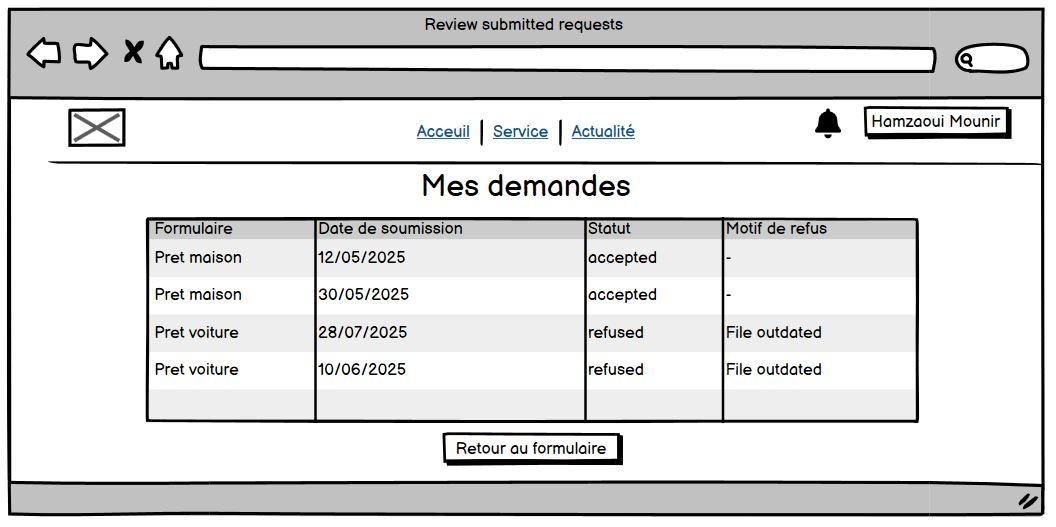
\includegraphics[width=0.9\textwidth]{figures/Tracksubstatus.JPG} 
    \caption{Prototype of Tracking the submission Page.}
\end{figure}\
 \begin{figure}[h]
    \centering
    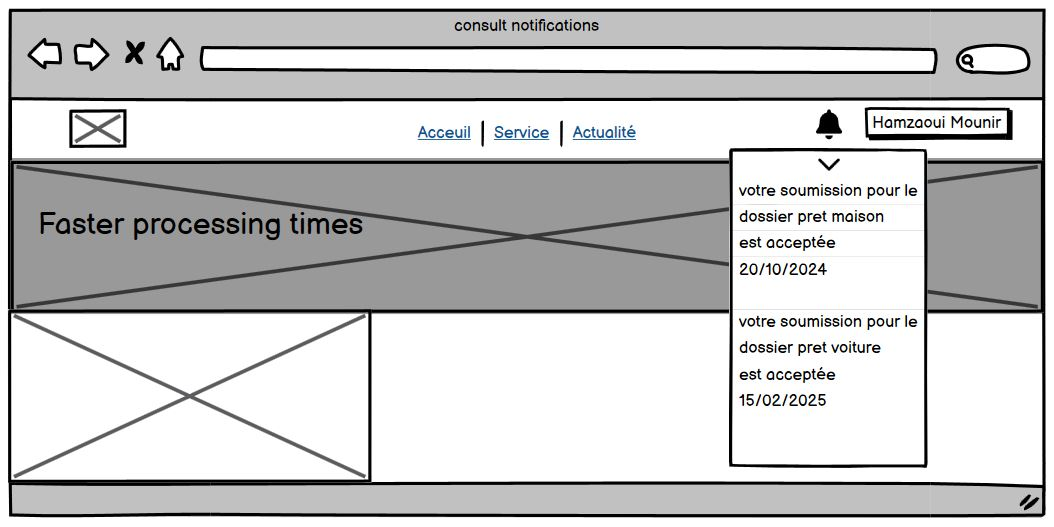
\includegraphics[width=0.9\textwidth]{figures/notifications.JPG}  
    \caption{Prototype of The notification drop-down.}
\end{figure}\
 \begin{figure}[h]
    \centering
    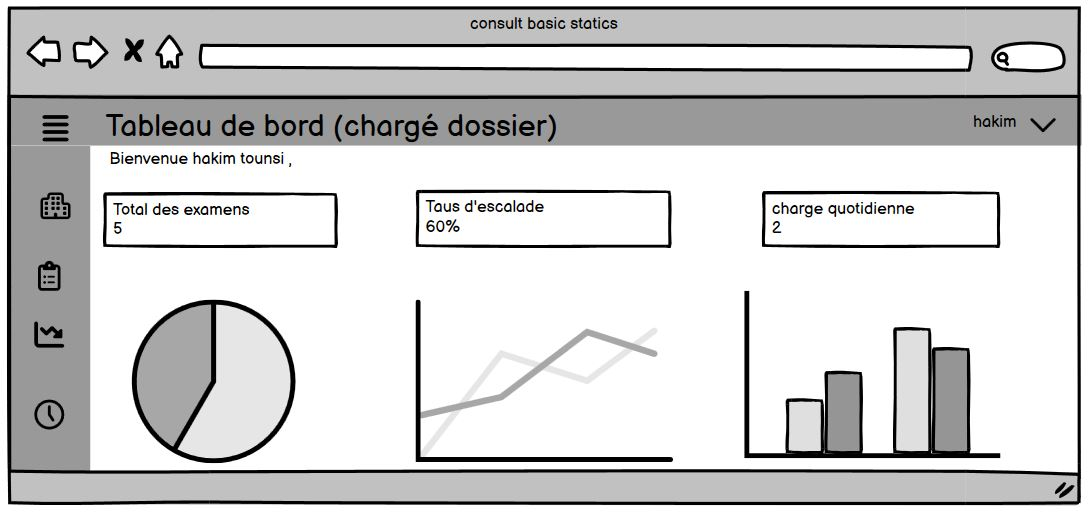
\includegraphics[width=0.9\textwidth]{figures/consult basic statics.JPG} 
    \caption{Prototype of consulting the basic statics Page.}
\end{figure}\
 \begin{figure}[h]
    \centering
    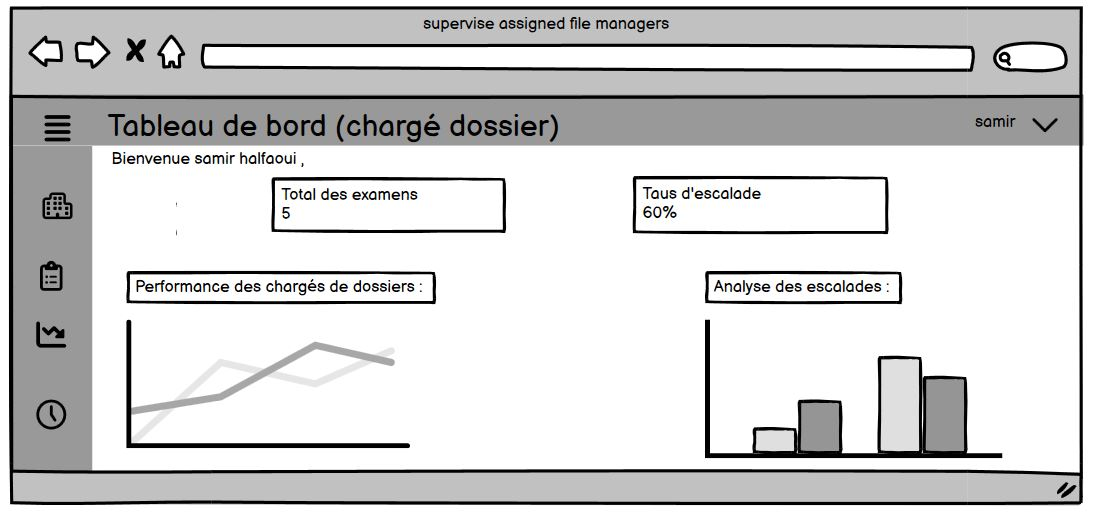
\includegraphics[width=0.9\textwidth]{figures/supervise assigned file managers.JPG} 
    \caption{Prototype of the supervision of the file managers Page.}
\end{figure}\
 \begin{figure}[h]
    \centering
    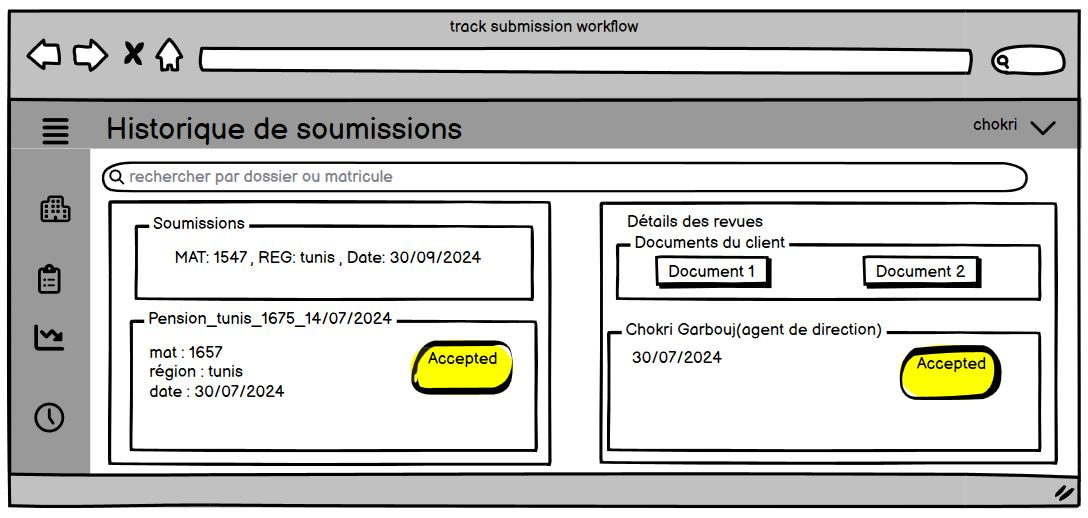
\includegraphics[width=0.9\textwidth]{figures/track sub workflow.JPG} 
    \caption{Prototype of Tracking the submission history Page.}
\end{figure}\
 \begin{figure}[h!]
    \centering
    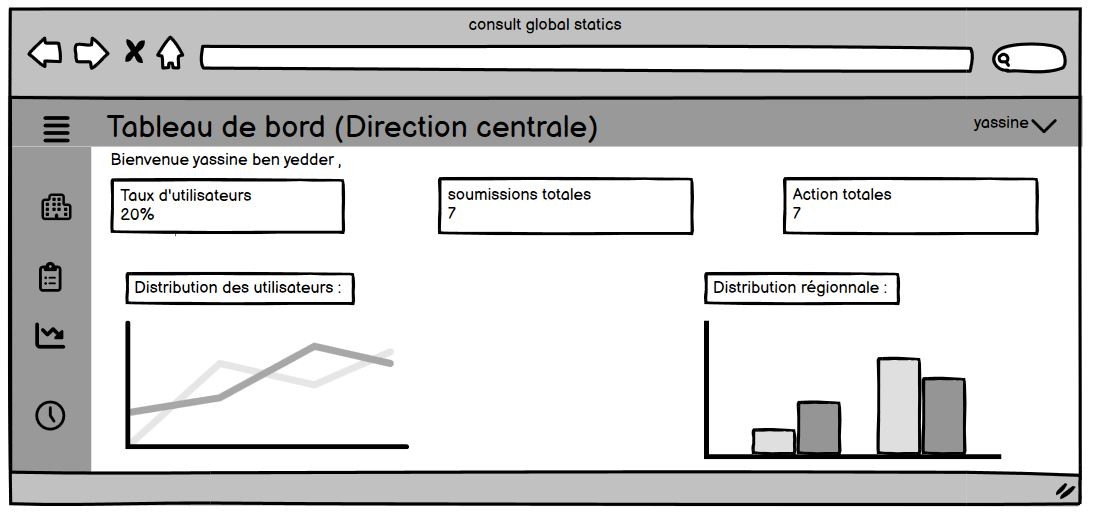
\includegraphics[width=0.9\textwidth]{figures/consult global statics.JPG}  % Replace with your image file
    \caption{Prototype of consulting the global statics Page.}
\end{figure}\

\section{Use Case Diagram of the Second Sprint}
This table provides a general classification of functionalities by actor.
 \begin{figure}[h]
    \centering
    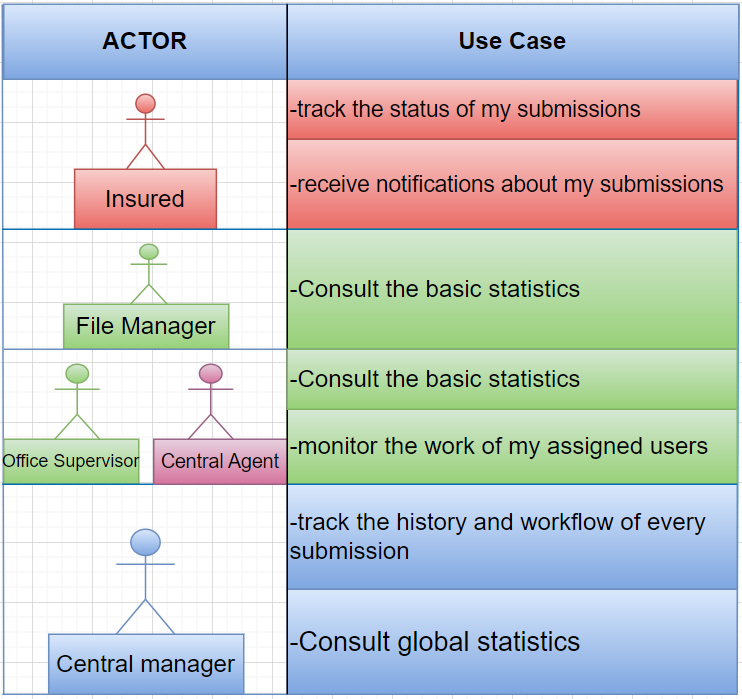
\includegraphics[width=0.6\textwidth]{figures/use case par acteur2.png}
    \caption{Classification of the use cases per actor.}
\end{figure}\
\begin{figure}[h!]
    \centering
    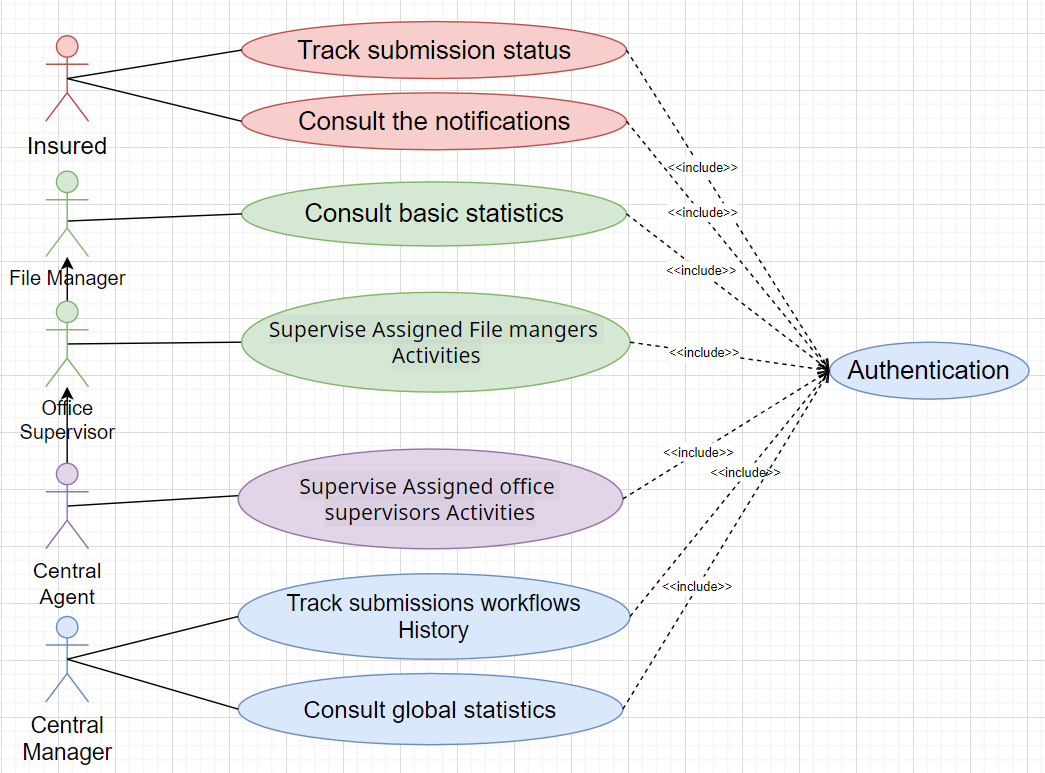
\includegraphics[width=0.9\textwidth]{figures/diagram use case s2.png}
    \caption{Use Case Diagram of the Second Sprint}
\end{figure}\
\newpage
\section{Use Case Analysis}
For each use case, we will provide a textual description in order to explain the scenario for each one and the exceptions that may arise.
\subsection{Use Case Analysis "Track submission status"}
\subsubsection{Textual Description of the "Track submission status" Use Case}
\begin{table}[h]
\centering
\begin{tabular}{|l|p{8cm}|}
\hline
\textbf{Use Case} & Track Submission Status \\ \hline
\textbf{Actor} & Insured \\ \hline
\textbf{Pre-condition} & The insured user is authenticated and sees the Dashboard option. \\ \hline
\textbf{Post-condition} & The system displays the list of submissions and their statuses. \\ \hline
\textbf{Main Scenario Description} & 
\begin{tabular}[c]{@{}l@{}}
1. The insured user clicks the "Dashboard"\\ element. \\
2. The system displays the list of submissions\\ and their statuses.
\end{tabular} \\ \hline
\textbf{Alternative Scenarios} & None specified. \\ \hline
\end{tabular}
\caption{Use Case: Track Submission Status}
\end{table}
\begin{figure}[h!]
    \centering
    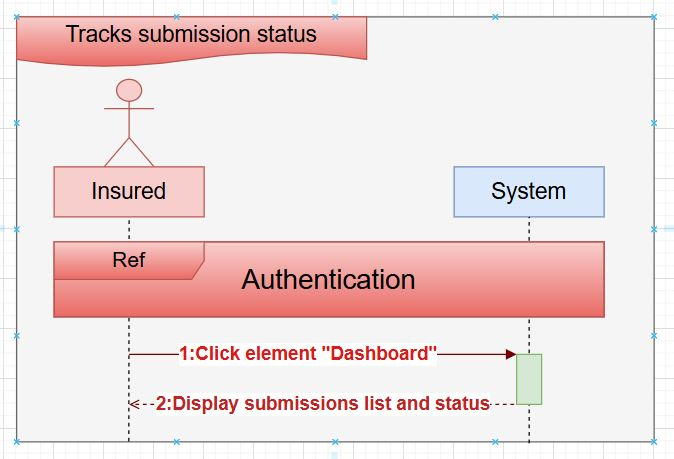
\includegraphics[width=0.9\textwidth]{figures/seq track sub status.JPG}
    \caption{Sequence Diagram of the use case 'Track submission status'}
\end{figure}\

\newpage
\subsection{Use Case Analysis "Consult the notifications"}
\subsubsection{Textual Description of the "Consult the notifications" Use Case}
\begin{table}[h]
\centering
\begin{tabular}{|l|p{8cm}|}
\hline
\textbf{Use Case} & Consult the Notifications \\ \hline
\textbf{Actor} & Insured \\ \hline
\textbf{Pre-condition} & The insured user is authenticated and has access to the notification alert button. \\ \hline
\textbf{Post-condition} & The system displays the list of notifications. \\ \hline
\textbf{Main Scenario Description} & 
\begin{tabular}[c]{@{}l@{}}
1. The insured user opens the Notification Alert\\ button. \\
2. The system displays the list of notifications.
\end{tabular} \\ \hline
\textbf{Alternative Scenarios} & None specified. \\ \hline
\end{tabular}
\caption{Use Case: Consult the Notifications}
\end{table}
\begin{figure}[h!]
    \centering
    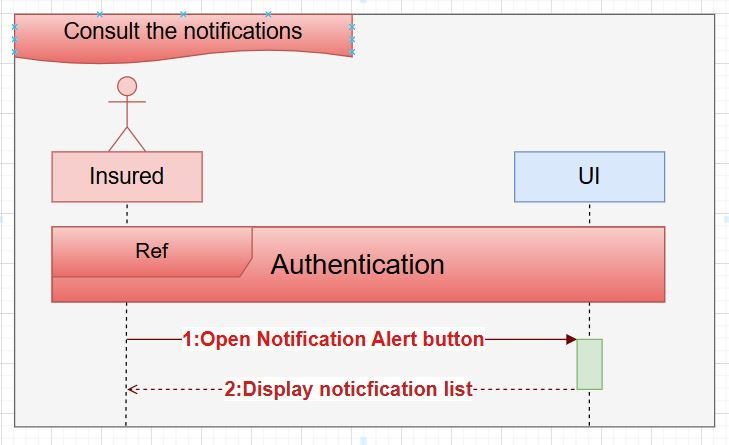
\includegraphics[width=0.9\textwidth]{figures/seq consult notifications.JPG}
    \caption{Sequence Diagram of the use case 'Consult the notifications'}
\end{figure}\

\newpage
\subsection{Use Case Analysis "Supervise Assigned File Managers"}
\subsubsection{Textual Description of the "Supervise Assigned File Managers" Use Case}
\begin{table}[h]
\centering
\begin{tabular}{|l|p{8cm}|}
\hline
\textbf{Use Case} & Supervise Assigned File Managers \\ \hline
\textbf{Actor} & Office Supervisor \\ \hline
\textbf{Pre-condition} & The supervisor is authenticated \\ \hline
\textbf{Post-condition} & The file managers team's performance is displayed. \\ \hline
\textbf{Main Scenario Description} & 
\begin{tabular}[c]{@{}l@{}}
1- The supervisor opens the supervision page.\\
2- The system displays the file managers team's \\performance.
\end{tabular} \\ \hline
\textbf{Alternative Scenarios} & None specified. \\ \hline
\end{tabular}
\caption{Use Case: Supervise Assigned File Managers}
\end{table}
\begin{figure}[h!]
    \centering
    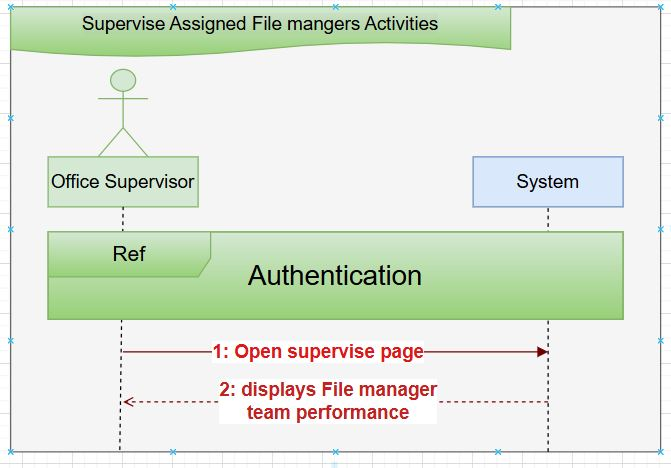
\includegraphics[width=0.9\textwidth]{figures/seq supervise assigned file managers activities.JPG}
    \caption{Sequence Diagram of the use case 'Supervise Assigned File Managers Activities'}
\end{figure}\

\newpage
\subsection{Use Case Analysis "Track Submissions Workflows History"}
\subsubsection{Textual Description of the "Track Submissions Workflows History" Use Case}
\begin{table}[h]
\centering
\begin{tabular}{|l|p{8cm}|}
\hline
\textbf{Use Case} & Track Submissions Workflows History \\ \hline
\textbf{Actor} & Central Manager \\ \hline
\textbf{Pre-condition} & The Central Manager is authenticated \\ \hline
\textbf{Post-condition} & The submission reviews and documents are displayed. \\ \hline
\textbf{Main Scenario Description} & 
\begin{tabular}[c]{@{}l@{}}
1- The central manager opens the history page.\\
2- The system displays the old submissions list.\\
3- The central manager clicks on a specific \\submission.\\
4- The system displays the submission reviews.\\
5- The central manager clicks on the "View \\Submission Documents" button.\\
6- The system displays the submission \\documents.
\end{tabular} \\ \hline
\textbf{Alternative Scenarios} & None specified. \\ \hline
\end{tabular}
\caption{Use Case: Track Submissions Workflows History}
\end{table}

\begin{figure}[h!]
    \centering
    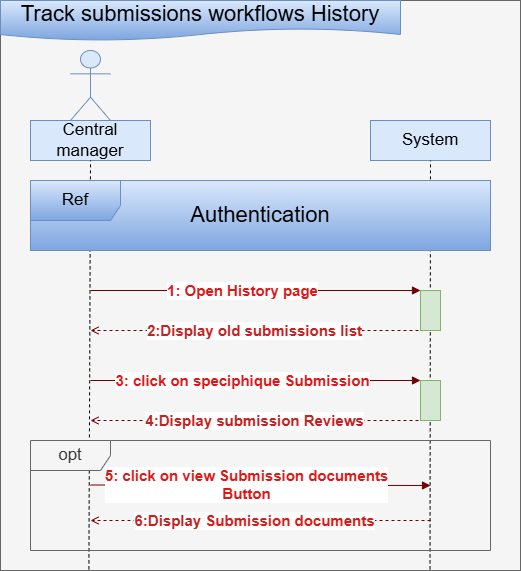
\includegraphics[width=1\textwidth]{figures/seq track sub workflow history.png}
    \caption{Sequence Diagram of the use case 'Track Submissions Workflows History'}
\end{figure}\

\clearpage
\subsection{Use Case Analysis "Consult Global Statistics"}
\subsubsection{Textual Description of the "Consult Global Statistics" Use Case}
\begin{table}[h]
\centering
\begin{tabular}{|l|p{8cm}|}
\hline
\textbf{Use Case} & Consult Global Statistics \\ \hline
\textbf{Actor} & Central Manager \\ \hline
\textbf{Pre-condition} & The Central Manager is authenticated \\ \hline
\textbf{Post-condition} & The performance dashboard and workload metrics are displayed. \\ \hline
\textbf{Main Scenario Description} & 
\begin{tabular}[c]{@{}l@{}}
1- The Central Manager opens the dashboard \\page.\\
2- The system displays the performance \\dashboard.\\
The Central Manager reviews the following \\statistics:\\
\quad - Review Decisions Distribution\\
\quad - Reviews by Reviewer\\
\quad - Submissions by Region\\
\quad - Status by Region\\
\quad - Submission Status\\
\quad - Form Type Distribution\\
\quad - Employee Distribution\\
\quad - Regional Employees\\
\quad - User Types\\
\quad - User Regions
\end{tabular} \\ \hline
\textbf{Alternative Scenarios} & None specified. \\ \hline
\end{tabular}
\caption{Use Case: Consult Global Statistics}
\end{table}
\begin{figure}[h!]
    \centering
    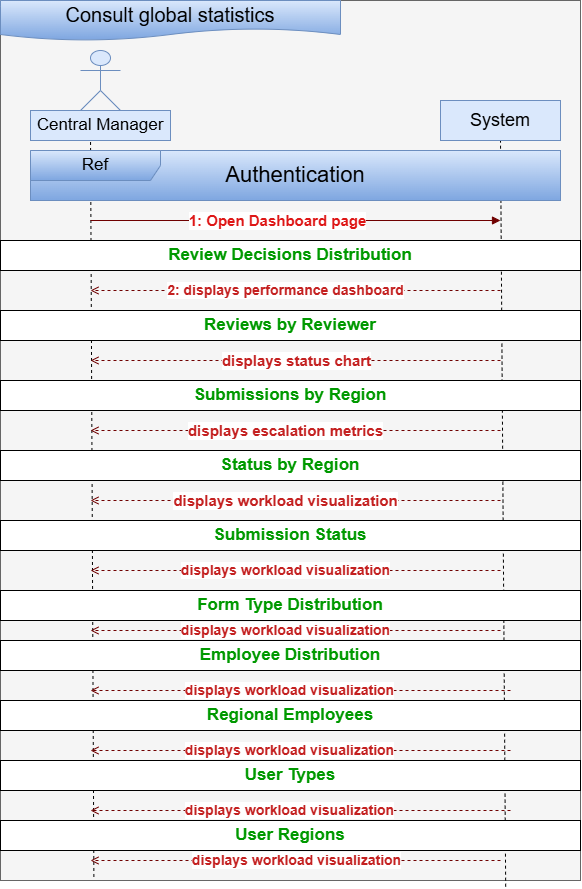
\includegraphics[width=1\textwidth]{figures/seq consult global statistics.png}
    \caption{Sequence Diagram of the use case 'Consult Global Statistics'}
\end{figure}\


\clearpage
\section{Design of Use Cases}
\subsection{The participant Class Diagram}
\subsubsection{Participant class Diagram for the use case "Track Submission Status"}
\begin{figure}[h!]
    \centering
    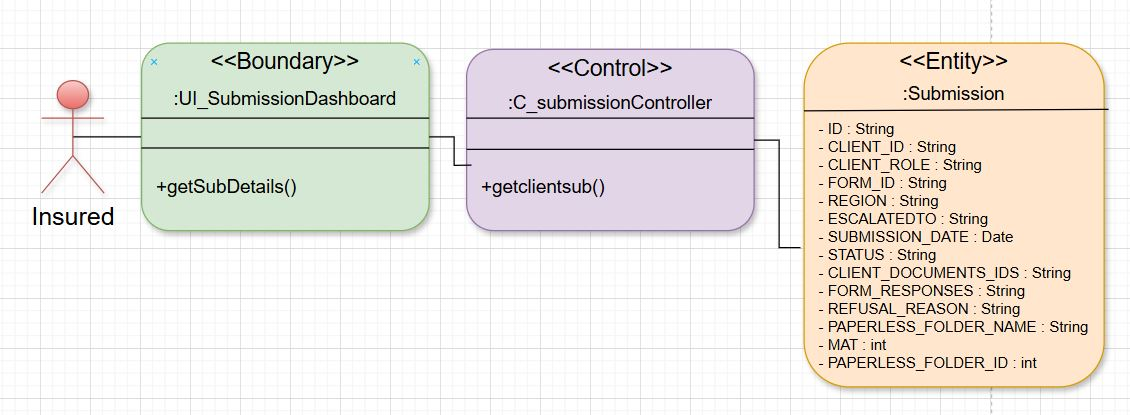
\includegraphics[width=1\textwidth]{figures/dc track sub status.JPG}
    \caption{Participant class Diagram for the use case "Track Submission Status"}
\end{figure}\

\subsubsection{Participant class Diagram for the use case "Consult Notifications"}
\begin{figure}[h!]
    \centering
    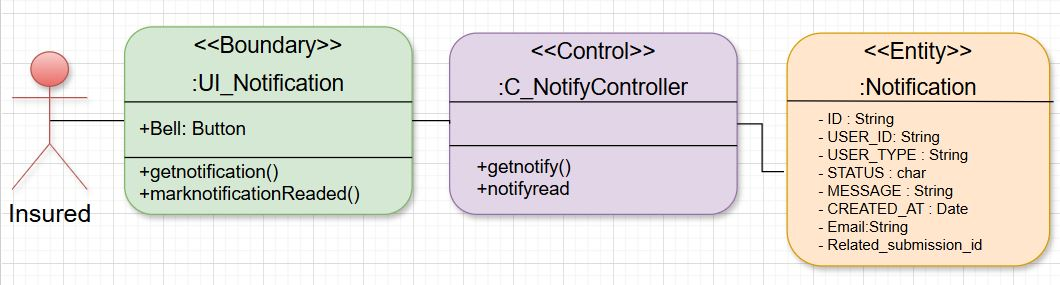
\includegraphics[width=1\textwidth]{figures/dc consult notifications.JPG}
    \caption{Participant class Diagram for the use case "Consult Notifications"}
\end{figure}\
\clearpage
\subsubsection{Participant class Diagram for the use case "Consult Basic Statistics"}
\begin{figure}[h!]
    \centering
    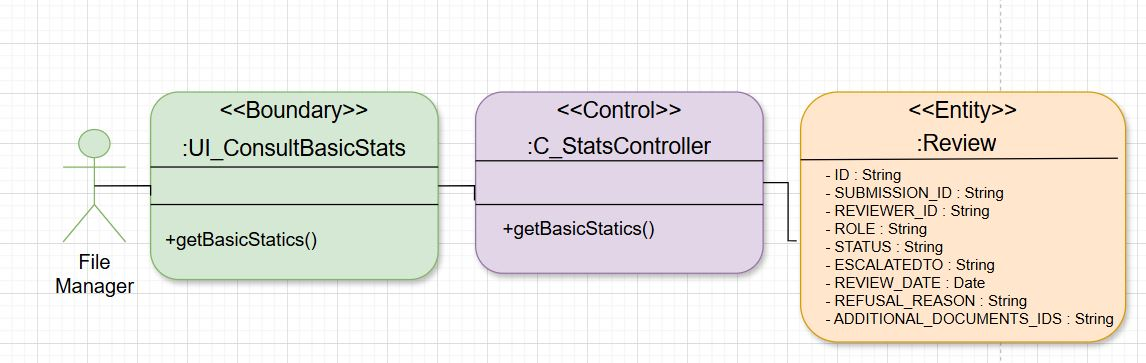
\includegraphics[width=1\textwidth]{figures/dc consult basic statistics.JPG}
    \caption{Participant class Diagram for the use case "Consult Basic Statistics"}
\end{figure}\
\subsubsection{Participant class Diagram for the use case "Supervise Assigned File Managers"}
\begin{figure}[h!]
    \centering
    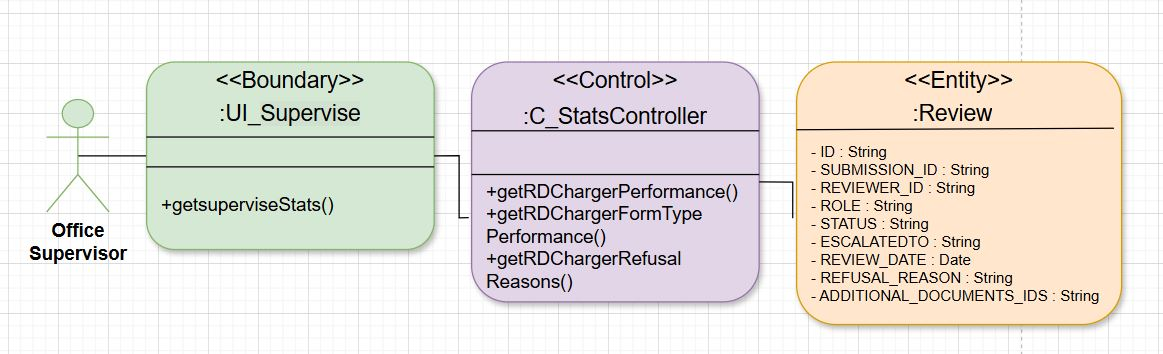
\includegraphics[width=1\textwidth]{figures/dc supervise assigned file managers activities.JPG}
    \caption{Participant class Diagram for the use case "Supervise Assigned File Managers"}
\end{figure}\
\clearpage
\subsubsection{Participant class Diagram for the use case "Track Submissions Workflows History"}
\begin{figure}[h!]
    \centering
    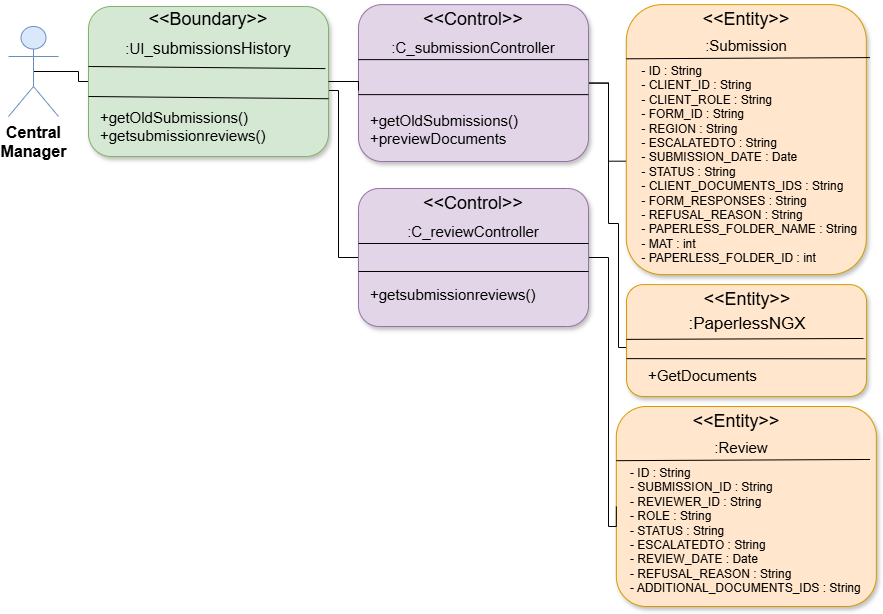
\includegraphics[width=1\textwidth]{figures/dc Track submissions Workflows history.png}
    \caption{Participant class Diagram for the use case "Track Submissions Workflows History"}
\end{figure}
\subsubsection{Participant class Diagram for the use case "Consult Global Statistics"}
\begin{figure}[h!]
    \centering
    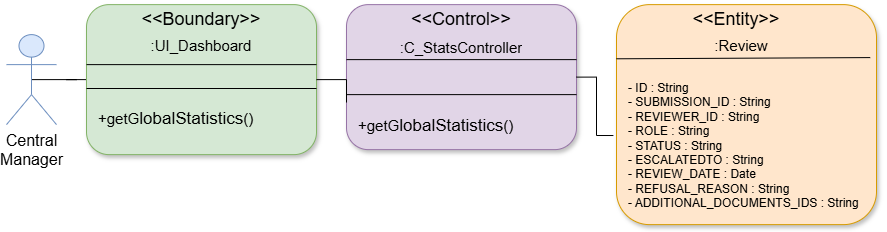
\includegraphics[width=1\textwidth]{figures/dc Consult global statistics.png}
    \caption{Participant class Diagram for the use case "Consult Global Statistics"}
\end{figure}
\clearpage
\subsection{Detailed Sequence Diagram}
\subsubsection{Detailed sequence diagram of the 'Track Submission Status' use case}
\begin{figure}[h!]
    \centering
    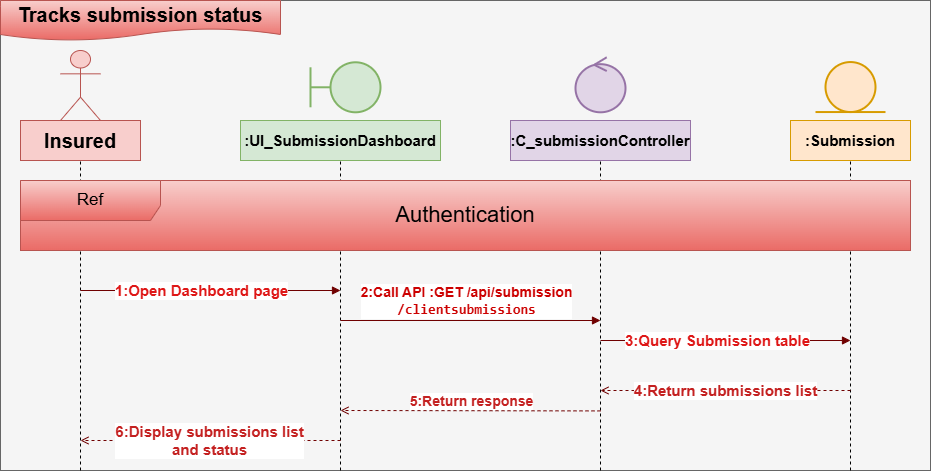
\includegraphics[width=1\textwidth]{figures/det Tracks submission status.png}
    \caption{Detailed sequence diagram of the 'Track Submission Status' use case}
\end{figure}
\subsubsection{Detailed sequence diagram of the 'Consult Notifications' use case}
\begin{figure}[h!]
    \centering
    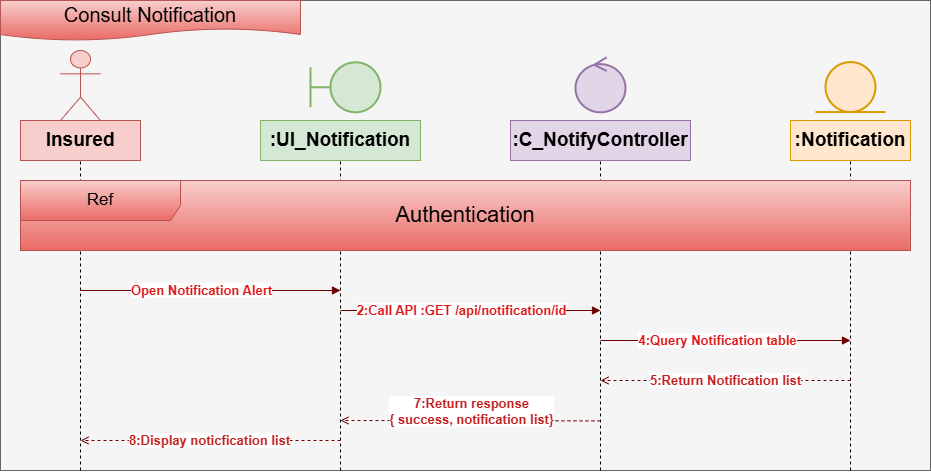
\includegraphics[width=1\textwidth]{figures/det consult notification.png}
    \caption{Detailed sequence diagram of the 'Consult Notifications' use case}
\end{figure}
\clearpage
\subsubsection{Detailed sequence diagram of the 'Consult Basic Statistics' use case}
\begin{figure}[h!]
    \centering
    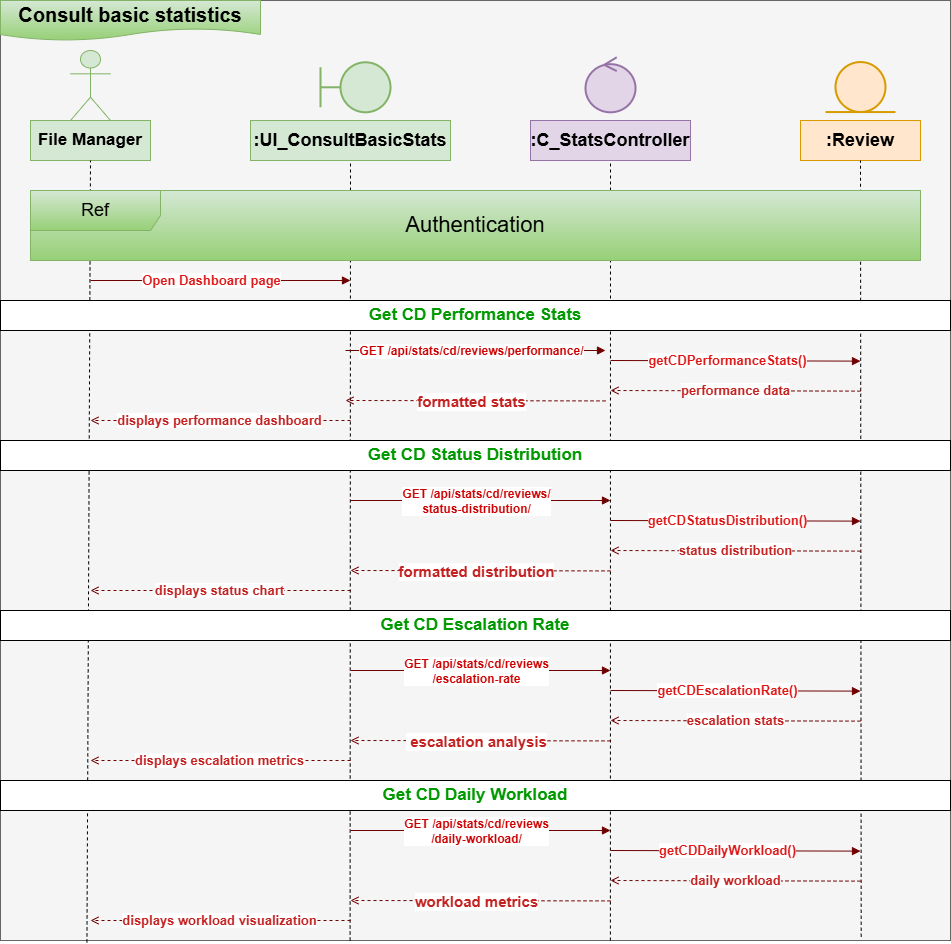
\includegraphics[width=1\textwidth]{figures/det consult basic stat.png}
    \caption{Detailed sequence diagram of the 'Consult Basic Statistics' use case}
\end{figure}
\clearpage
\subsubsection{Detailed sequence diagram of the 'Supervise Assigned File Managers Activities' use case}
\begin{figure}[h!]
    \centering
    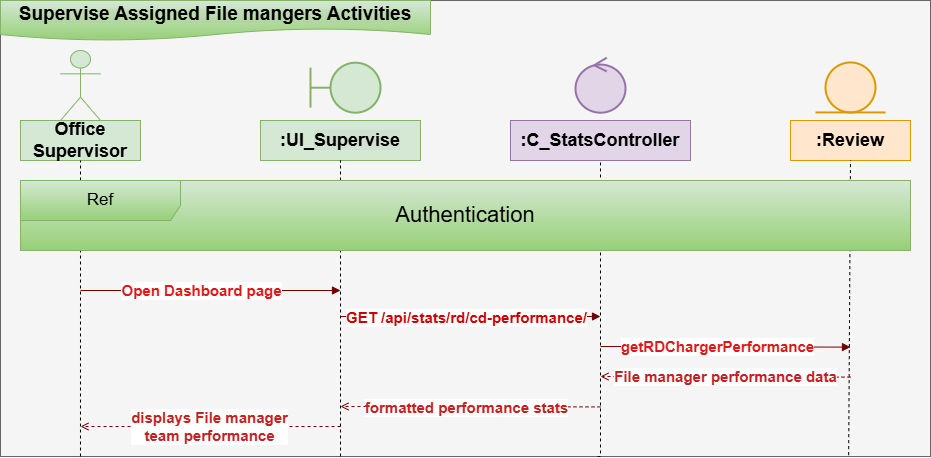
\includegraphics[width=1\textwidth]{figures/det supervise assigned file managers activities.png}
    \caption{Detailed sequence diagram of the 'Supervise Assigned File Managers Activities' use case}
\end{figure}
\subsubsection{Detailed sequence diagram of the 'Track Submissions Workflow History' use case}
\begin{figure}[h!]
    \centering
    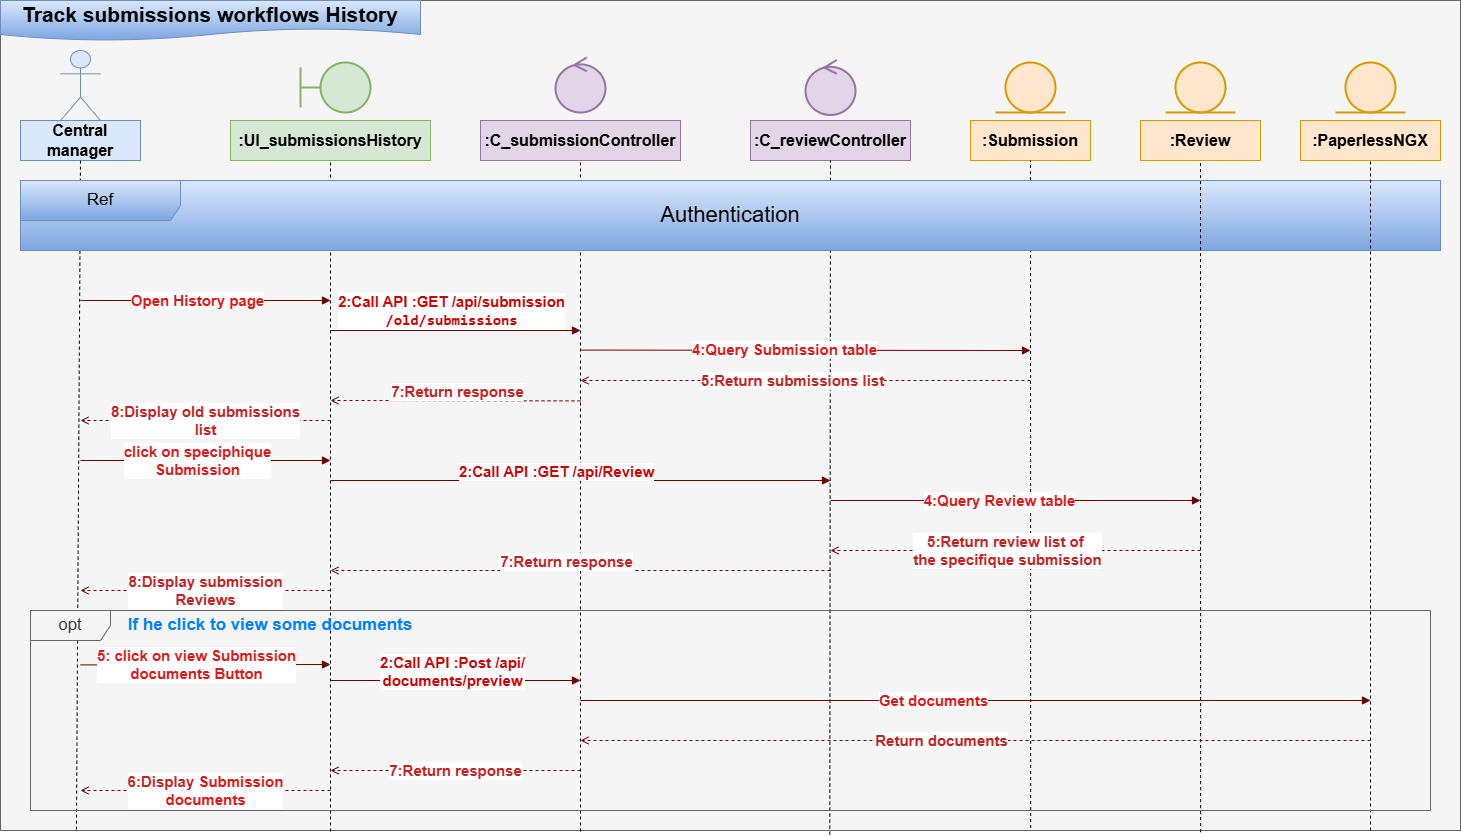
\includegraphics[width=1\textwidth]{figures/det track sub workflow history.png}
    \caption{Detailed sequence diagram of the 'Track Submissions Workflow History' use case}
\end{figure}
\clearpage

\subsubsection{Detailed sequence diagram of the 'Consult Global Statistics' use case}
\begin{figure}[h!]
    \centering
    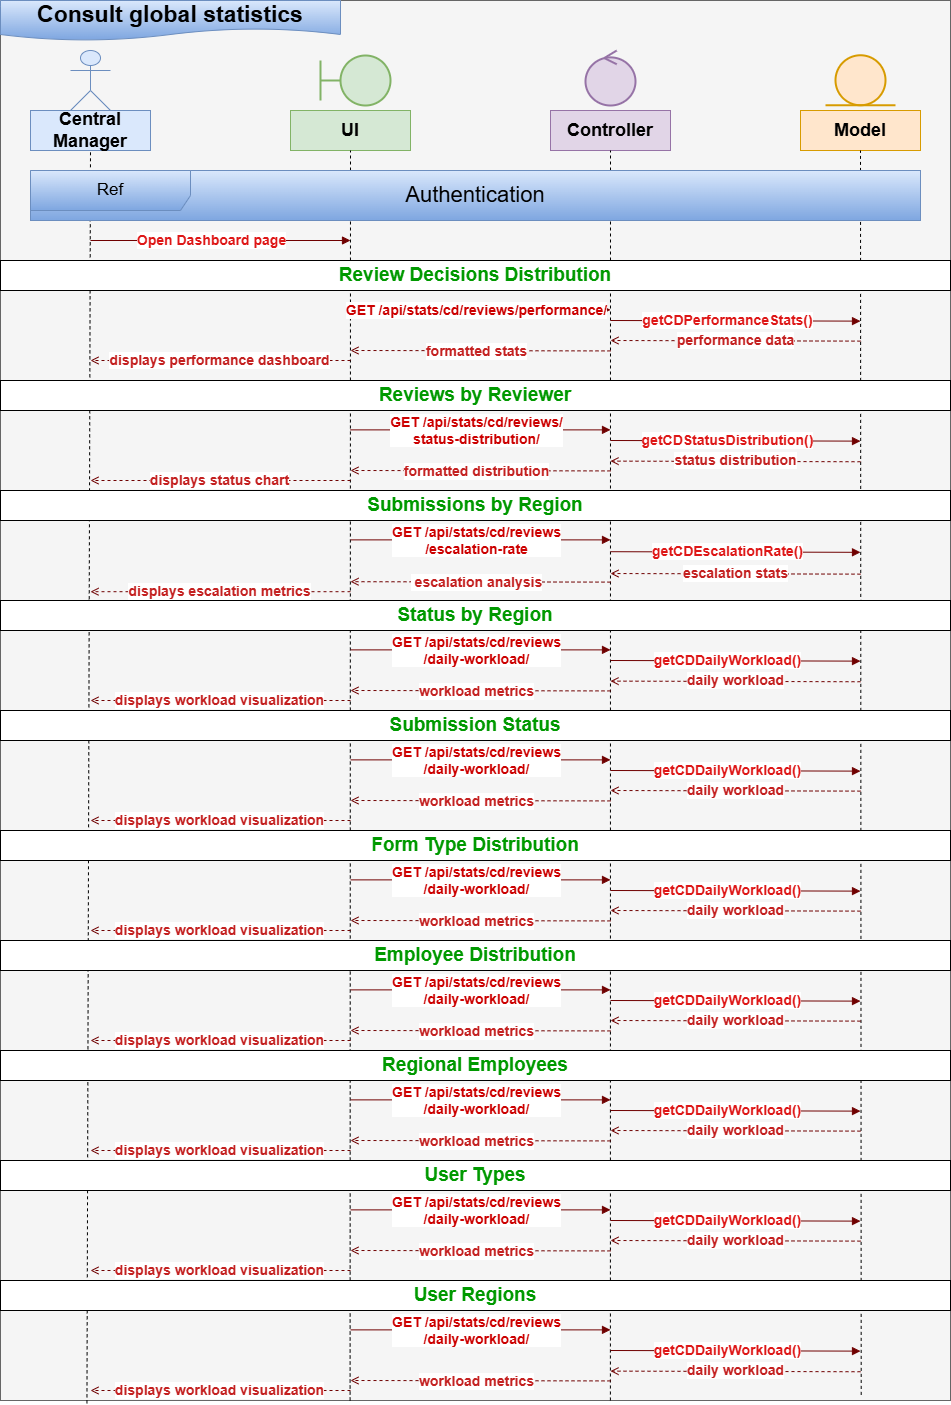
\includegraphics[width=1\textwidth]{figures/det consult global statistics.png}
    \caption{Detailed sequence diagram of the 'Consult Global Statistics' use case}
\end{figure}

\section{Global class diagram of the second sprint}
\begin{figure}[h!]
    \centering
    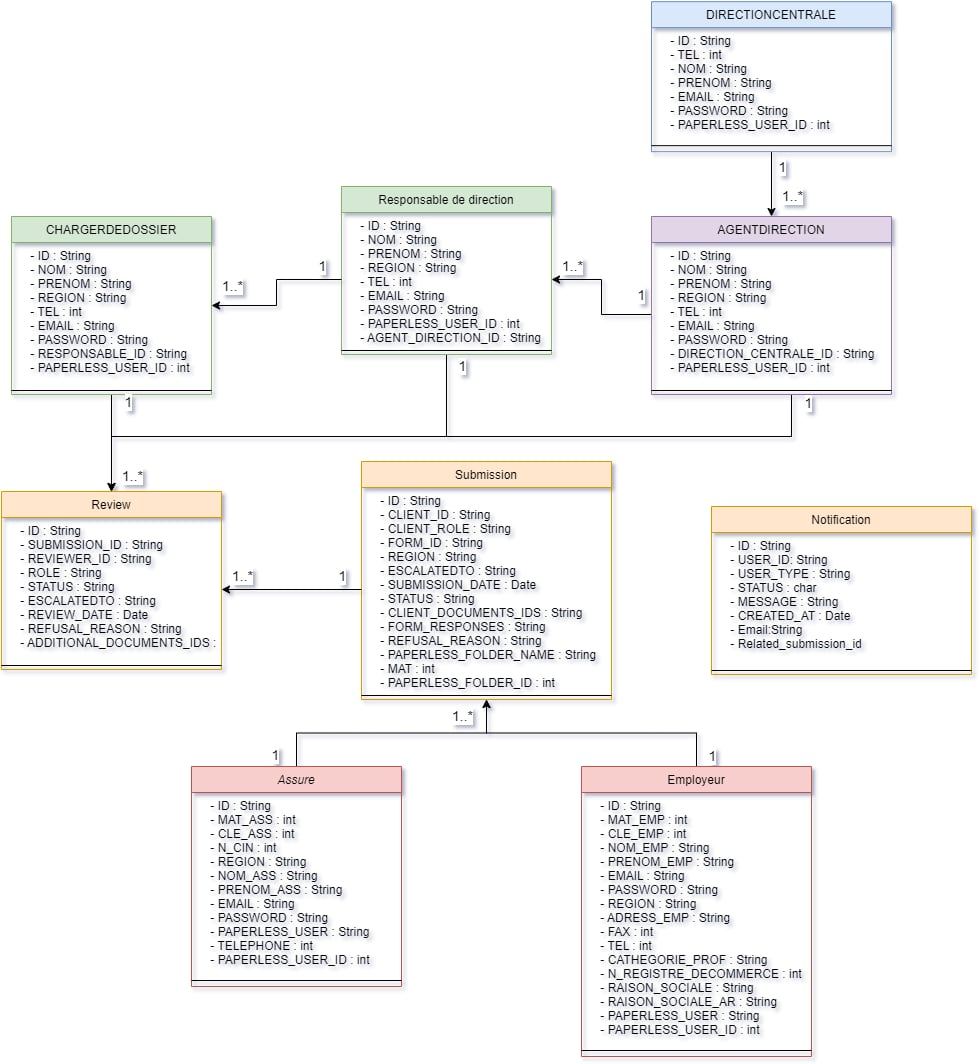
\includegraphics[width=1\textwidth]{figures/global class dia s2.jpg}
    \caption{Global class diagram of Sprint 2.}
\end{figure}
\clearpage
\section{Implementation}
In this step, we will define the structure of the current sprint's database while applying the rules for transforming the entity/association model into the relational model.
\subsection{The Database Schemas}
\begin{table}[h!]
\centering
\begin{tabular}{|l|l|l|}
\hline
\textbf{Attribut} & \textbf{Type} & \textbf{Contrainte} \\
\hline
ID & VARCHAR & PRIMARY KEY \\
NOM & VARCHAR(50) & Not Null \\
PRENOM & VARCHAR(50) & Not Null \\
REGION & VARCHAR(50) & - \\
TEL & VARCHAR(15) & - \\
EMAIL & VARCHAR(100) & UNIQUE - Not Null \\
PASSWORD & VARCHAR(255) & Not Null \\
RESPONSABLE\_ID & VARCHAR & FOREIGN KEY - Not Null \\
PAPERLESS\_USER\_ID & INT & FOREIGN KEY - Not Null \\
\hline
\end{tabular}
\caption{Table \texttt{CHARGERDEDOSSIER}}
\end{table}
\begin{table}[h!]
\centering
\begin{tabular}{|l|l|l|}
\hline
\textbf{Attribut} & \textbf{Type} & \textbf{Contrainte} \\
\hline
ID & VARCHAR & PRIMARY KEY \\
NOM & VARCHAR(50) & Not Null \\
PRENOM & VARCHAR(50) & Not Null \\
REGION & VARCHAR(50) & - \\
TEL & VARCHAR(15) & - \\
EMAIL & VARCHAR(100) & UNIQUE - Not Null \\
PASSWORD & VARCHAR(255) & Not Null \\
PAPERLESS\_USER\_ID & INT & FOREIGN KEY - Not Null \\
AGENT\_DIRECTION\_ID & VARCHAR & FOREIGN KEY \\
\hline
\end{tabular}
\caption{Table \texttt{ResponsableDirection}}
\end{table}
\clearpage
\begin{table}[h!]
\centering
\begin{tabular}{|l|l|l|}
\hline
\textbf{Attribut} & \textbf{Type} & \textbf{Contrainte} \\
\hline
ID & VARCHAR & PRIMARY KEY \\
NOM & VARCHAR(50) & Not Null \\
PRENOM & VARCHAR(50) & Not Null \\
REGION & VARCHAR(50) & - \\
TEL & VARCHAR(15) & - \\
EMAIL & VARCHAR(100) & UNIQUE - Not Null \\
PASSWORD & VARCHAR(255) & Not Null \\
DIRECTION\_CENTRALE\_ID & VARCHAR & FOREIGN KEY \\
PAPERLESS\_USER\_ID & INT & FOREIGN KEY - Not Null \\
\hline
\end{tabular}
\caption{Table \texttt{AgentDirection}}
\end{table}
\begin{table}[h!]
\centering
\begin{tabular}{|l|l|l|}
\hline
\textbf{Attribut} & \textbf{Type} & \textbf{Contrainte} \\
\hline
ID & VARCHAR & PRIMARY KEY \\
TEL & INT & - \\
NOM & VARCHAR(50) & Not Null \\
PRENOM & VARCHAR(50) & Not Null \\
EMAIL & VARCHAR(100) & UNIQUE - Not Null \\
PASSWORD & VARCHAR(255) & Not Null \\
PAPERLESS\_USER\_ID & INT & FOREIGN KEY - Not Null \\
\hline
\end{tabular}
\caption{Table \texttt{DirectionCentrale}}
\end{table}
\begin{table}[h!]
\centering
\begin{tabular}{|l|l|l|}
\hline
\textbf{Attribut} & \textbf{Type} & \textbf{Contrainte} \\
\hline
ID & VARCHAR & PRIMARY KEY \\
CLIENT\_ID & VARCHAR & FOREIGN KEY \\
CLIENT\_ROLE & VARCHAR(50) & Not Null \\
FORM\_ID & VARCHAR & FOREIGN KEY \\
REGION & VARCHAR(50) & - \\
ESCALATEDTO & VARCHAR & - \\
SUBMISSION\_DATE & DATE & Not Null \\
STATUS & VARCHAR(20) & Not Null \\
CLIENT\_DOCUMENTS\_IDS & VARCHAR(255) & - \\
FORM\_RESPONSES & TEXT & - \\
REFUSAL\_REASON & TEXT & - \\
PAPERLESS\_FOLDER\_NAME & VARCHAR(255) & - \\
MAT & INT & - \\
PAPERLESS\_FOLDER\_ID & INT & FOREIGN KEY - Not Null \\
\hline
\end{tabular}
\caption{Table \texttt{Submission}}
\end{table}
\clearpage
\begin{table}[h]
\centering
\begin{tabular}{|l|l|l|}
\hline
\textbf{Attribute} & \textbf{Type} & \textbf{Constraint} \\ \hline
ID & VARCHAR2(36) & PRIMARY KEY \\ \hline
USER\_ID & VARCHAR2(36) & Not Null \\ \hline
USER\_TYPE & VARCHAR2(20) & Check: 'assure' or 'employeur' \\ \hline
MESSAGE & VARCHAR2(2000) & Not Null \\ \hline
STATUS & VARCHAR2(20) & Check: 'unread' or 'read' \\ \hline
CREATED\_AT & DATE & Default: SYSDATE \\ \hline
RELATED\_SUBMISSION\_ID & VARCHAR2(36) & FOREIGN KEY \\ \hline
EMAIL & VARCHAR2(20) & Default: 'undone' \\ \hline
\end{tabular}
\caption{Table "NOTIFICATION"}
\end{table}
\begin{table}[h!]
\centering
\begin{tabular}{|l|l|l|}
\hline
\textbf{Attribut} & \textbf{Type} & \textbf{Contrainte} \\
\hline
ID & VARCHAR & PRIMARY KEY \\
SUBMISSION\_ID & VARCHAR & FOREIGN KEY \\
REVIEWER\_ID & VARCHAR & FOREIGN KEY \\
ROLE & VARCHAR(50) & - \\
STATUS & VARCHAR(50) & - \\
ESCALATEDTO & VARCHAR & - \\
REVIEW\_DATE & DATE & - \\
REFUSAL\_REASON & TEXT & - \\
ADDITIONAL\_DOCUMENTS\_IDS & TEXT & - \\
\hline
\end{tabular}
\caption{Table \texttt{Review}}
\end{table}

\begin{table}[h!]
\centering
\begin{tabular}{|l|l|l|}
\hline
\textbf{Attribut} & \textbf{Type} & \textbf{Contrainte} \\
\hline
ID & VARCHAR & PRIMARY KEY \\
MAT\_ASS & INT & UNIQUE - Not Null \\
CLE\_ASS & INT & - \\
REGION & VARCHAR(50) & - \\
NOM\_ASS & VARCHAR(50) & Not Null \\
PRENOM\_ASS & VARCHAR(50) & Not Null \\
EMAIL & VARCHAR(100) & UNIQUE - Not Null \\
PASSWORD & VARCHAR(255) & Not Null \\
PAPERLESS\_USER\_ID & INT & FOREIGN KEY - Not Null \\
TELEPHONE & INT & - \\
\hline
\end{tabular}
\caption{Table \texttt{Assure}}
\end{table}
\clearpage
\begin{table}[h!]
\centering
\begin{tabular}{|l|l|l|}
\hline
\textbf{Attribut} & \textbf{Type} & \textbf{Contrainte} \\
\hline
ID & VARCHAR & PRIMARY KEY \\
MAT\_EMP & INT & UNIQUE - Not Null \\
CLE\_EMP & INT & - \\
NOM\_EMP & VARCHAR(50) & Not Null \\
PRENOM\_EMP & VARCHAR(50) & Not Null \\
EMAIL & VARCHAR(100) & UNIQUE - Not Null \\
PASSWORD & VARCHAR(255) & Not Null \\
REGION & VARCHAR(50) & - \\
ADRESSE\_EMP & TEXT & - \\
FAX & INT & - \\
TEL & INT & - \\
CATEGORIE\_PROF & VARCHAR(50) & - \\
N\_REGISTRE\_DECOMMERCE & VARCHAR(50) & - \\
RAISON\_SOCIALE & VARCHAR(255) & - \\
RAISON\_SOCIALE\_AR & VARCHAR(255) & - \\
PAPERLESS\_USER\_ID & INT & FOREIGN KEY - Not Null \\
\hline
\end{tabular}
\caption{Table \texttt{Employeur}}
\end{table}
\subsection{The interfaces of the use cases}
\begin{figure}[h!]
    \centering
    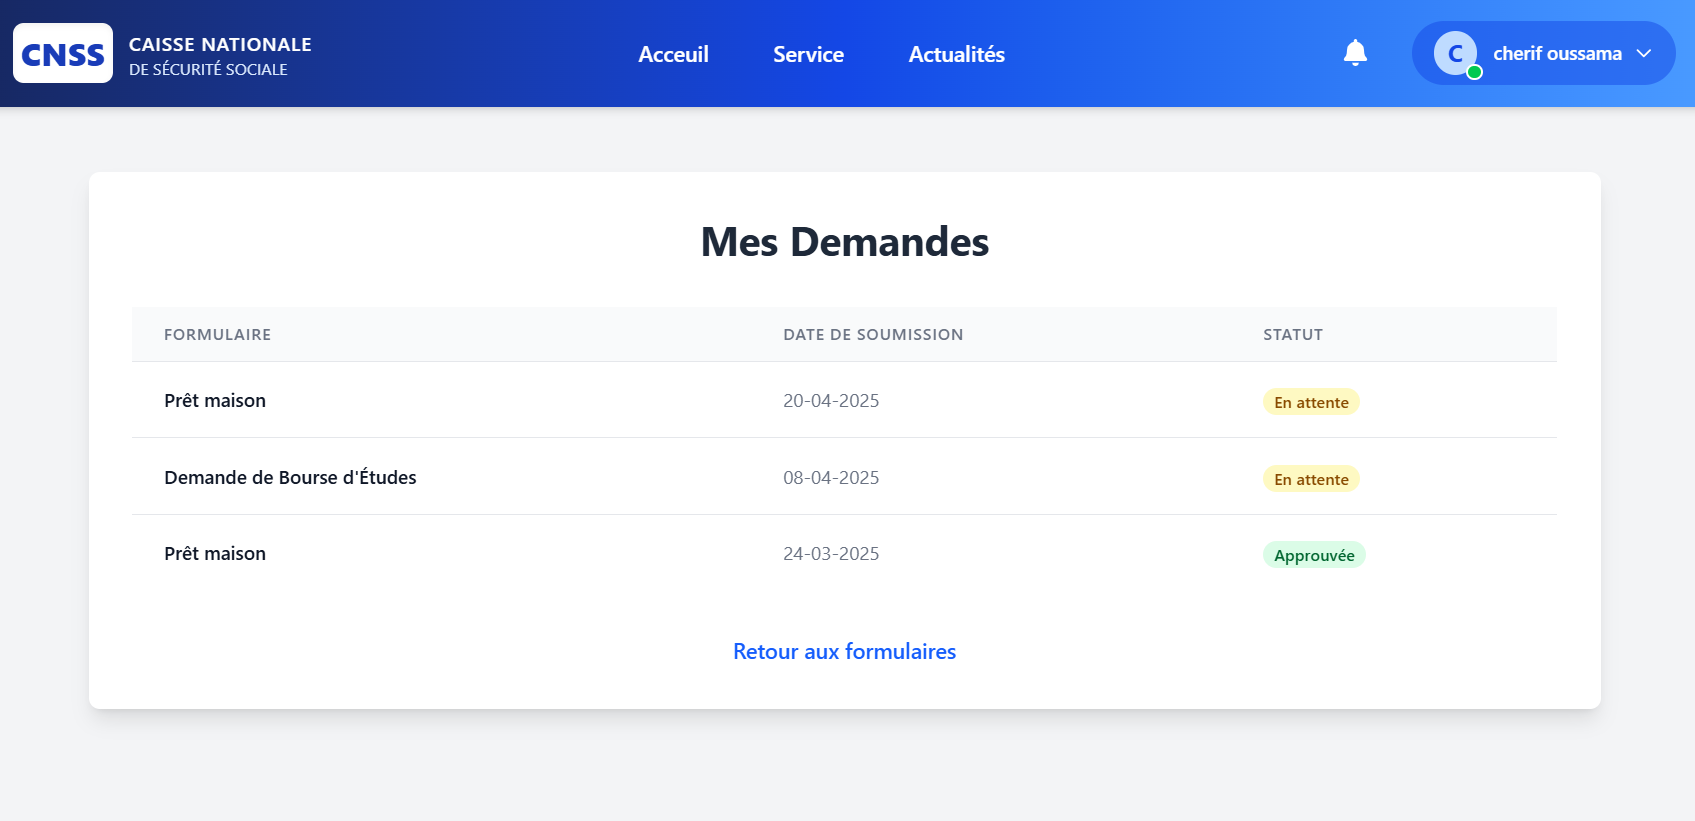
\includegraphics[width=1\textwidth]{figures/ui-track sub status.png}
    \caption{Interface of Tracking submissions status page.}
\end{figure}


\begin{figure}[h!]
    \centering
    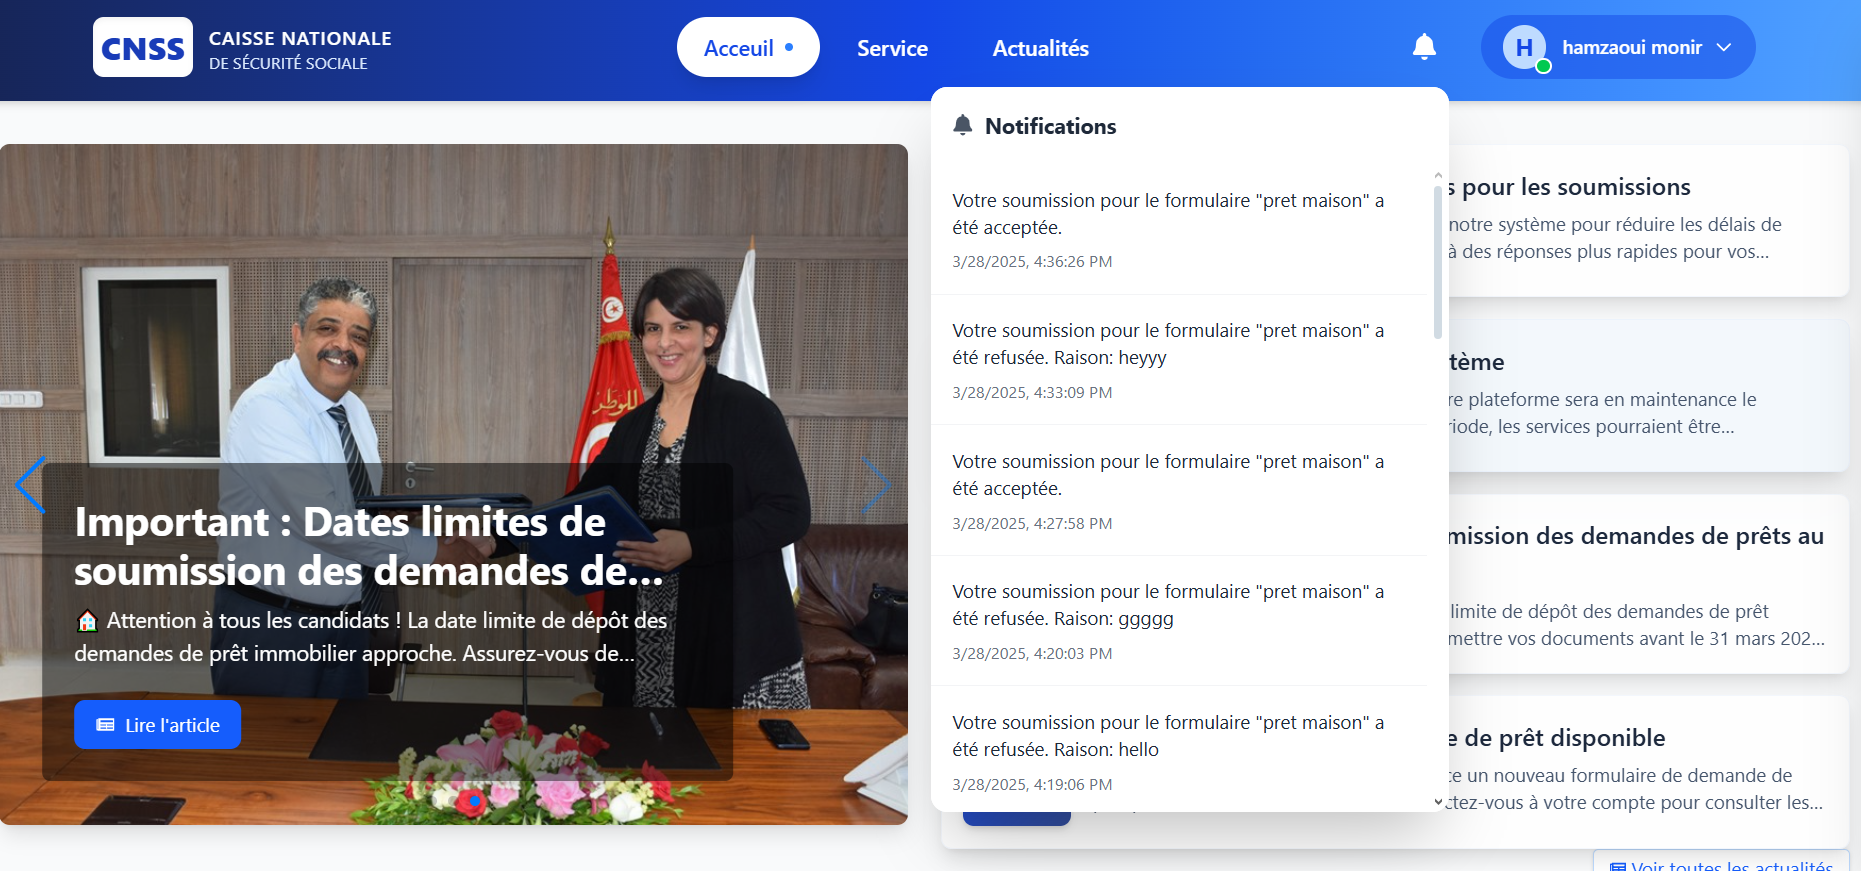
\includegraphics[width=1\textwidth]{figures/ui-consult notif.png}
    \caption{Interface of the Notification drop-down.}
\end{figure}
\begin{figure}[h!]
    \centering
    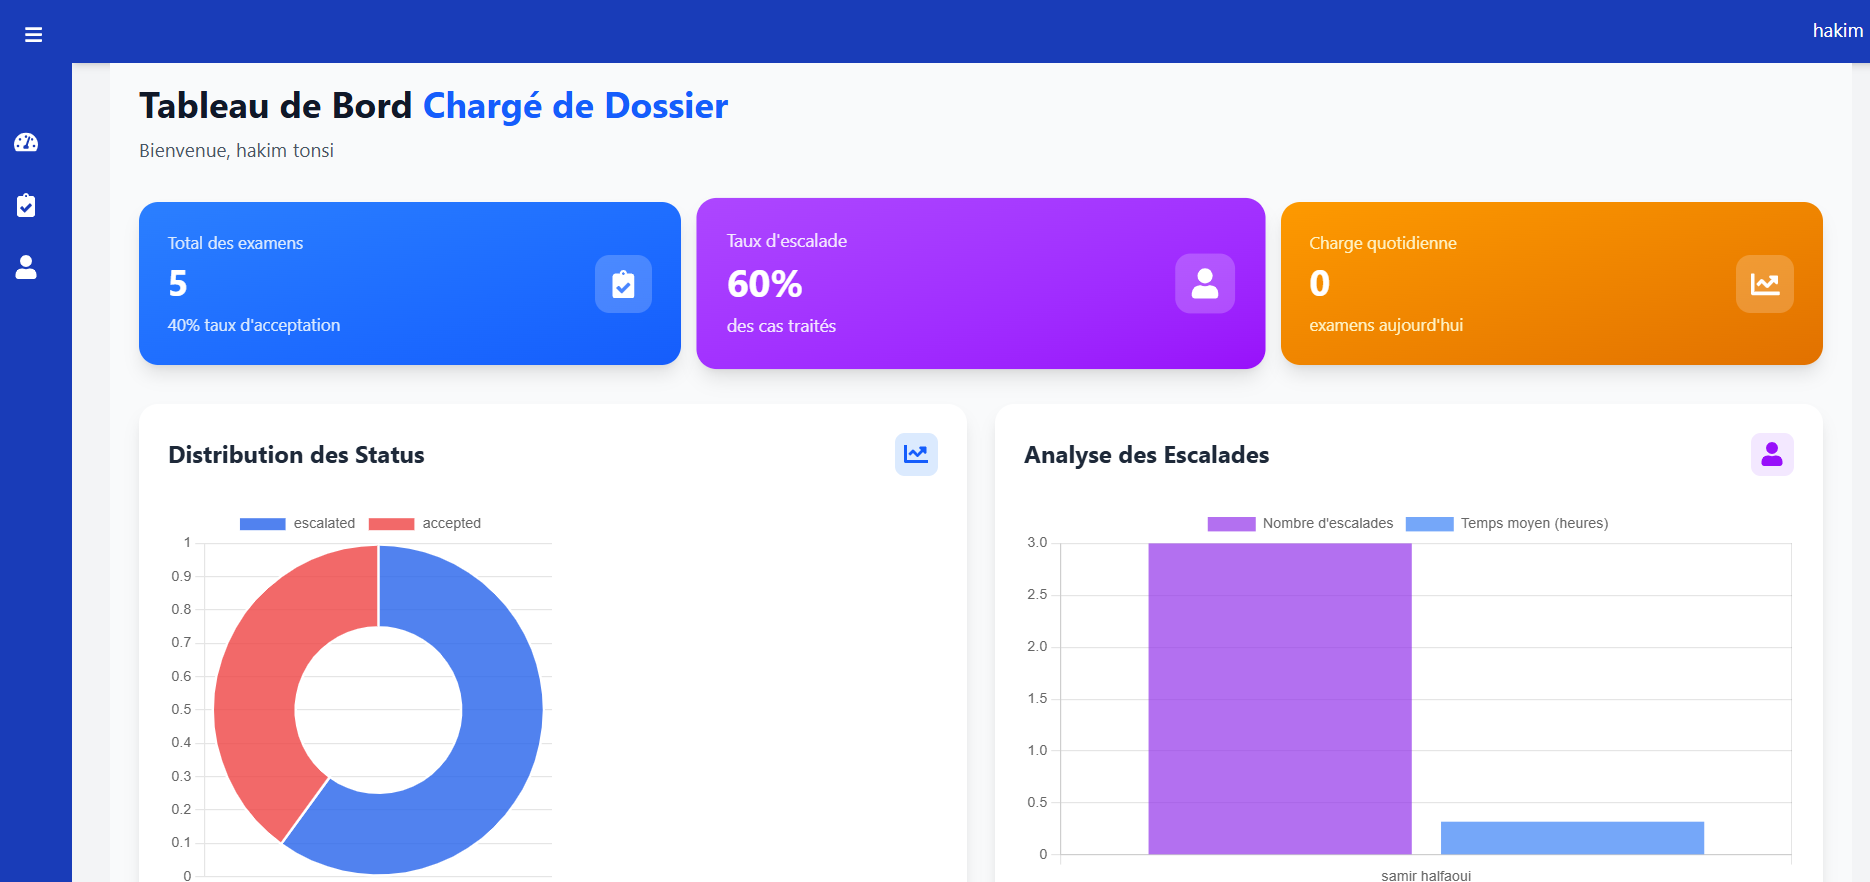
\includegraphics[width=1\textwidth]{figures/ui-consult basic stat.png}
    \caption{Interface of the basic statistics Page.}
\end{figure}
\begin{figure}[h!]
    \centering
    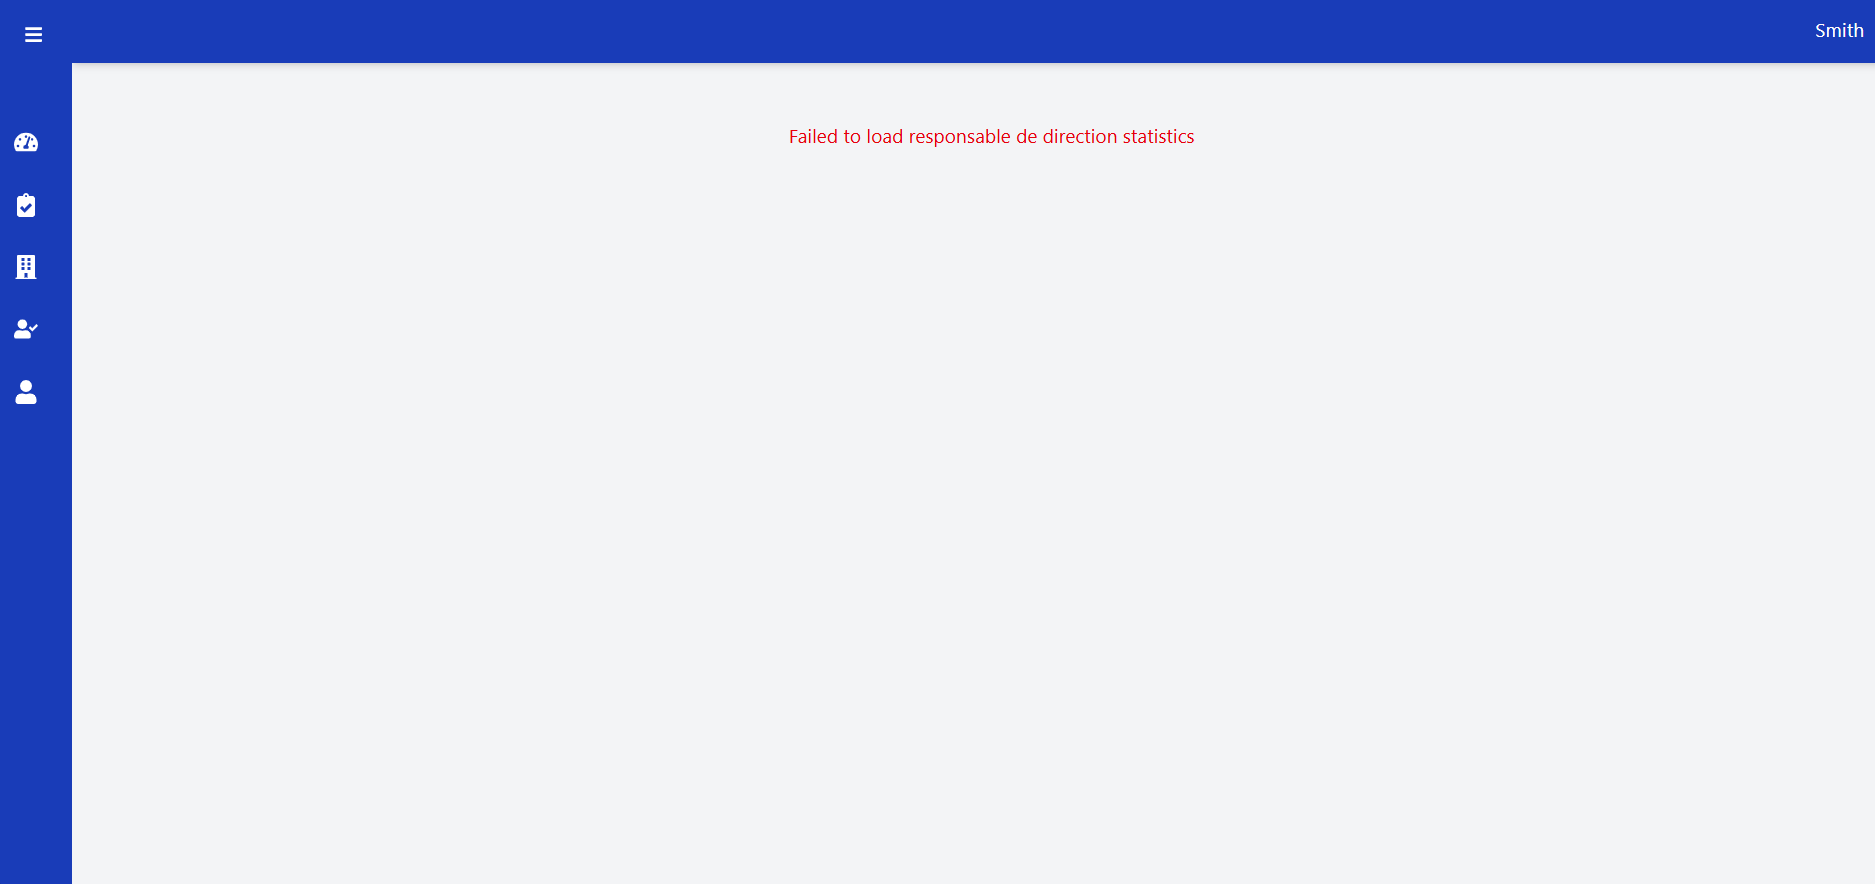
\includegraphics[width=1\textwidth]{figures/ui-supervise assigned fl activities.png}
    \caption{Interface of supervising the file managers activities Page.}
\end{figure}
\begin{figure}[h!]
    \centering
    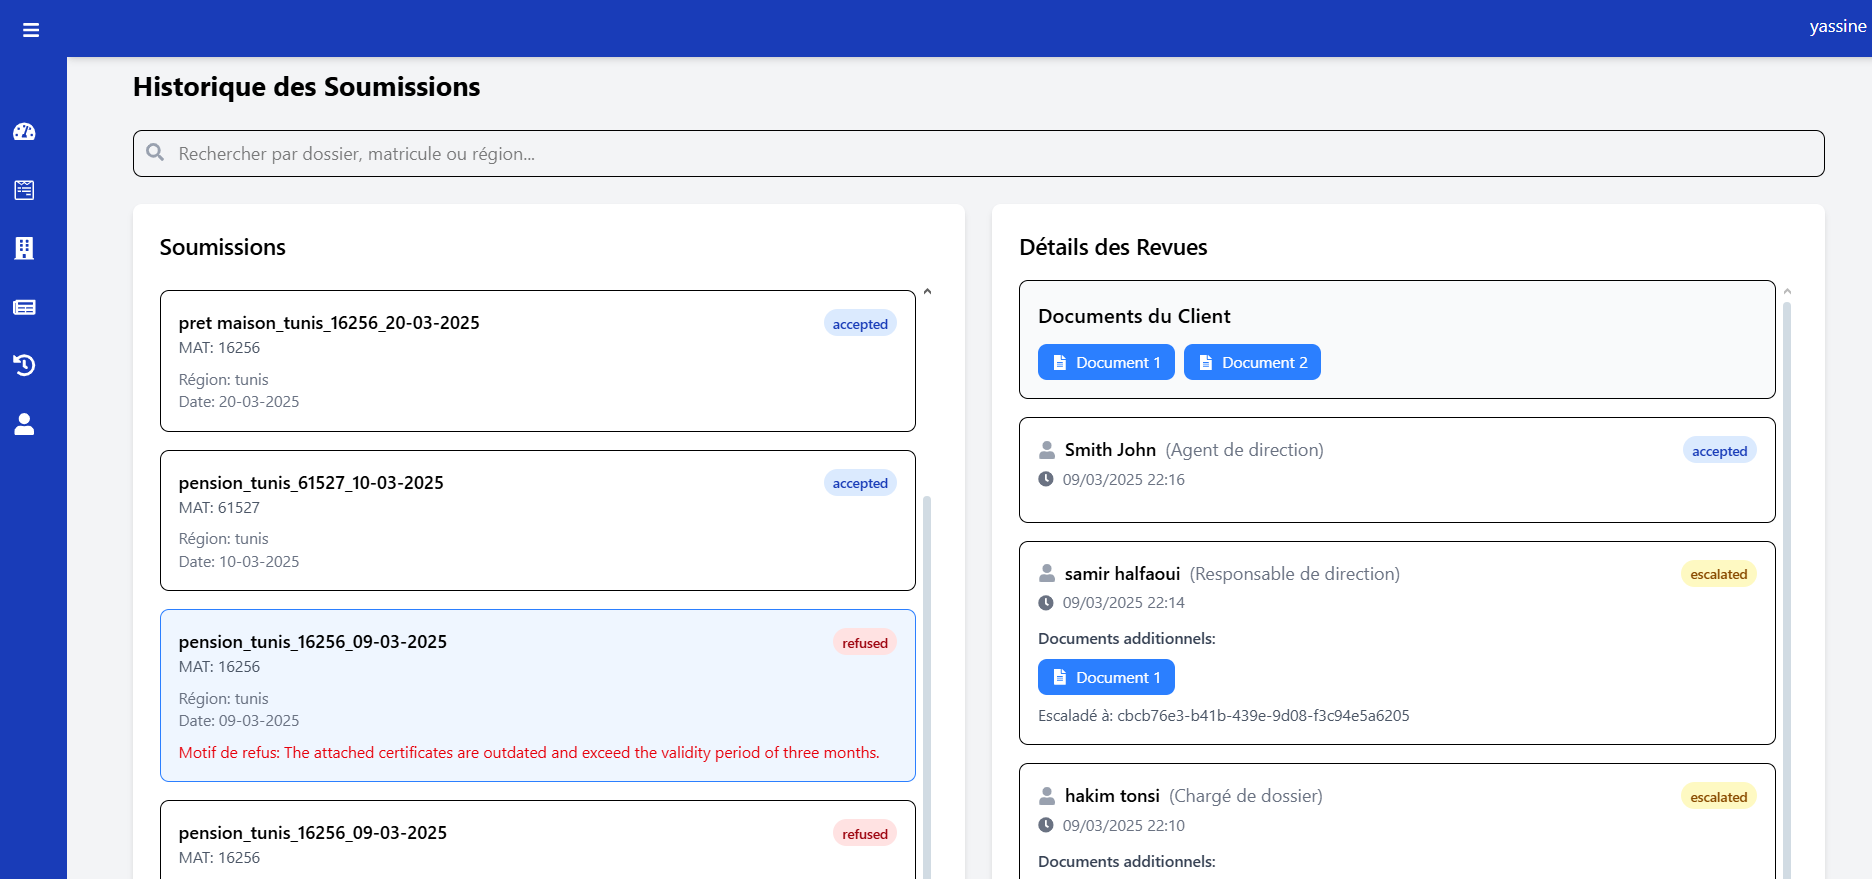
\includegraphics[width=1\textwidth]{figures/ui-track workflow history.png}
    \caption{Interface of tracking the workflow history Page.}
\end{figure}
\begin{figure}[h!]
    \centering
    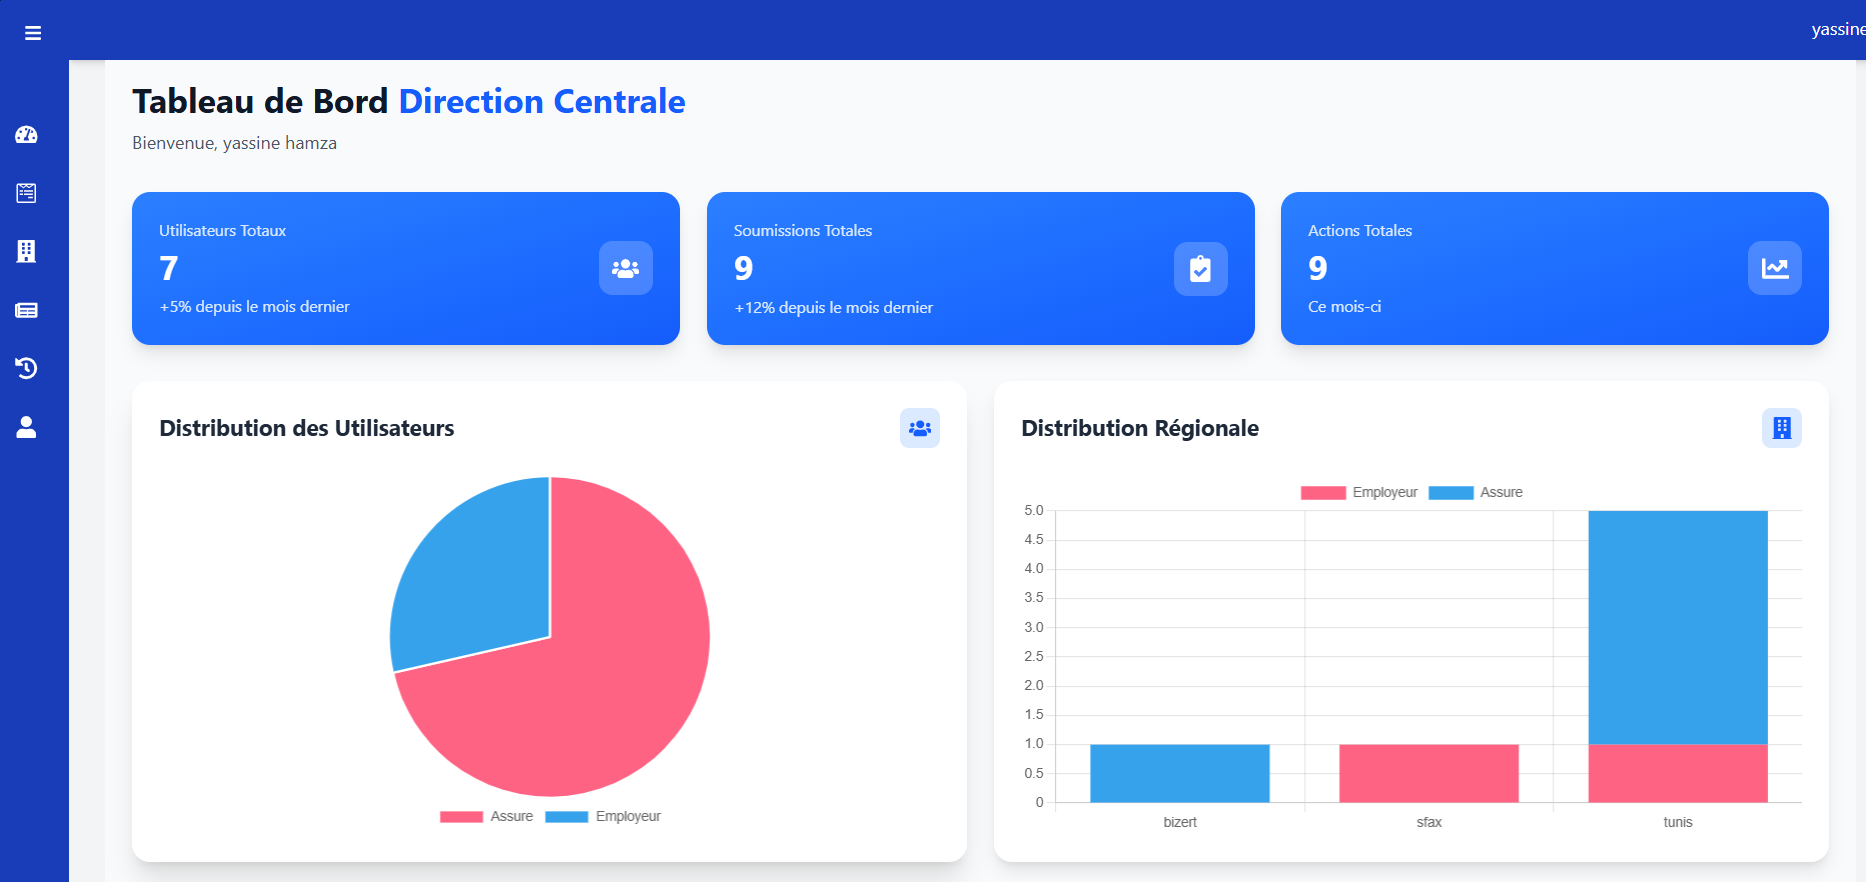
\includegraphics[width=1\textwidth]{figures/ui-consult global stat.png}
    \caption{Interface of the Global statistics Page.}
\end{figure}
\clearpage
\section{Tests}
During this phase, we will compare the expected results with the actual results.
This will give us the opportunity to ensure the proper functioning of the units (methods) previously implemented.
\subsection{Unit Testing}
We continue to work with the open source Jest unit testing framework to demonstrate in this section some examples of unit tests performed, along with the reasoning behind their implementation.

\subsection{ Unit Test for the Use Case "Track submission status"}
\subsubsection{Reasoning}
To test the tracking of the submission status request, we followed the reasoning below:
\begin{itemize}
    \item Create an object of type SuiviSoumission (SubmissionTracking).
    \item Set the attributes of the object with relevant information (e.g., candidate ID, submission ID, status, date of update).
    \item Simulate or retrieve a submission status update from the database.
    \item Test whether the tracking data is correctly retrieved and reflects the expected status.
\end{itemize}
\subsubsection{Successful Test Case "Track submission status"} 
In the case of success, the test performed should return a positive result.
\begin{figure}[h!]
    \centering
    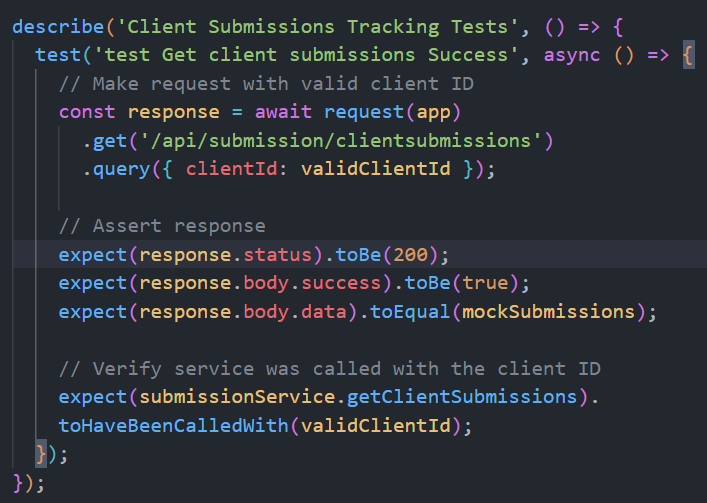
\includegraphics[width=1\textwidth]{figures/track subS code.png} 
    \caption{Source code of the method track submission status.}
\end{figure} \
\begin{figure}[h!]
    \centering
    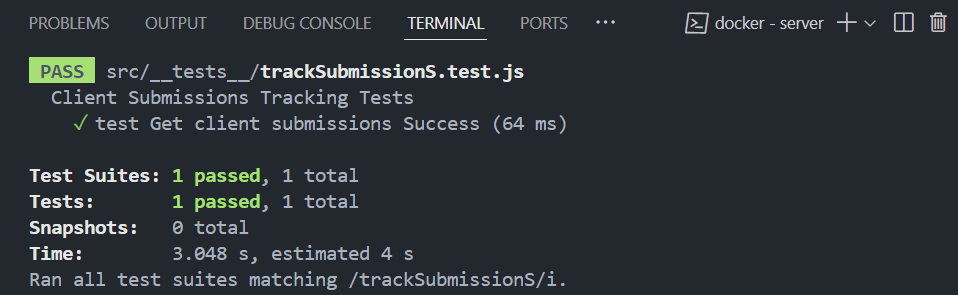
\includegraphics[width=1\textwidth]{figures/result tracksubS.png}  
    \caption{Result of the test tracking the submission status.}
\end{figure} \
\clearpage
\subsubsection{Failure Test Case "Track submission status"}
In the case of a fail, the test performed should return a negative result.
\begin{figure}[h!]
    \centering
    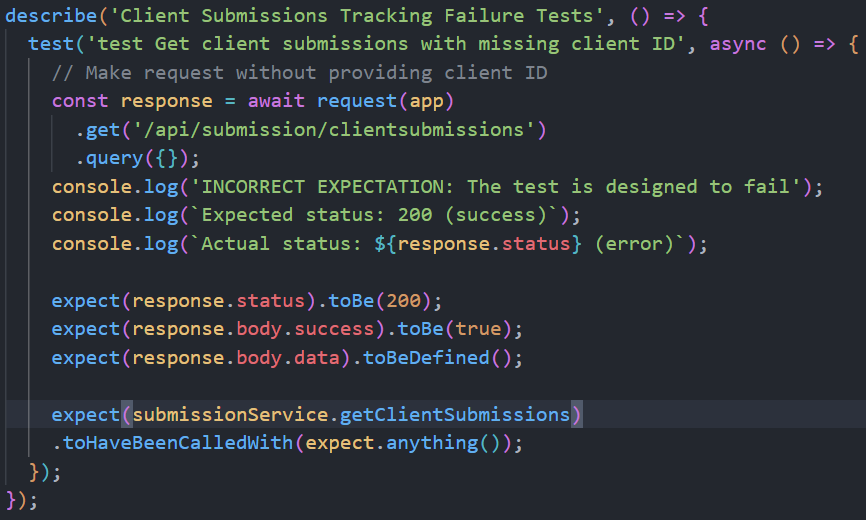
\includegraphics[width=1\textwidth]{figures/track subF code.png}
    \caption{Source code of the method track submission status.}
\end{figure} \
\begin{figure}[h!]
    \centering
    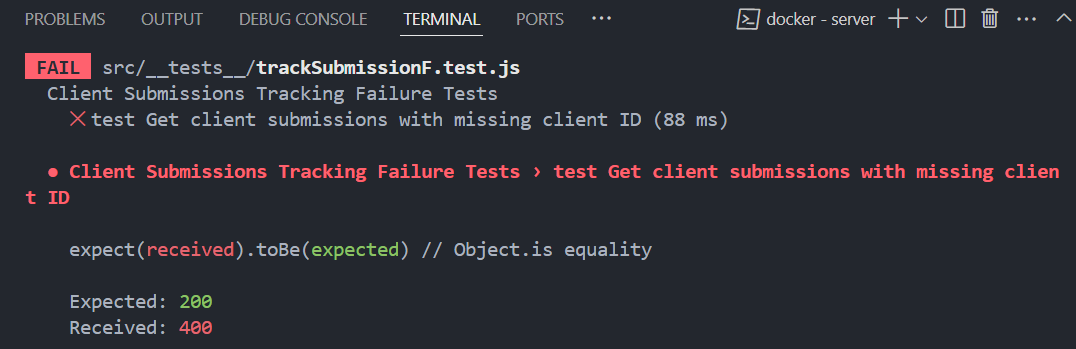
\includegraphics[width=1\textwidth]{figures/result tracksubF.png}  
    \caption{Result of the test tracking the submission status.}
\end{figure} \
\clearpage

\subsection{ Unit Test for the Use Case "Consult Notifications"}
\subsubsection{Reasoning}
To test consulting notifications request, we followed the reasoning below:
\begin{itemize}
    \item Create an object of type Notification.
    \item Set the necessary attributes (e.g., user ID, message content, status: read/unread, date).
    \item Simulate fetching notifications for a specific user from the database.
    \item Test whether the correct list of notifications is retrieved and if their statuses (e.g., unread) are accurately represented.
\end{itemize}
\subsubsection{Successful Test Case "Consult notifications"} 
In the case of success, the test performed should return a positive result.
\begin{figure}[h!]
    \centering
    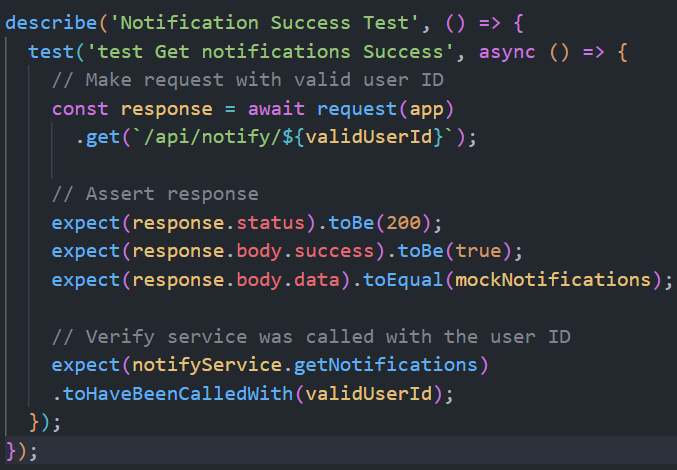
\includegraphics[width=1\textwidth]{figures/consult notifS code.png} 
    \caption{Source code of the method consult notifications.}
\end{figure} \
\begin{figure}[h]
    \centering
    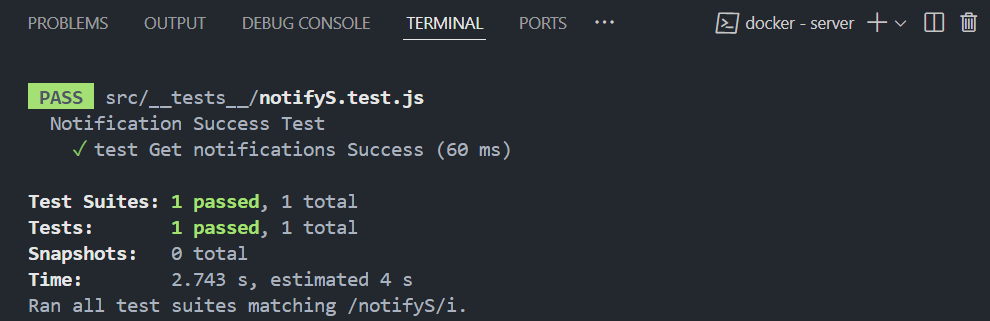
\includegraphics[width=1\textwidth]{figures/result consult notifS.png}  
    \caption{Result of the test consulting notifications.}
\end{figure} \
\
\subsubsection{Failure Test Case "Consult notifications"}
In the case of a fail, the test performed should return a negative result.
\begin{figure}[h!]
    \centering
    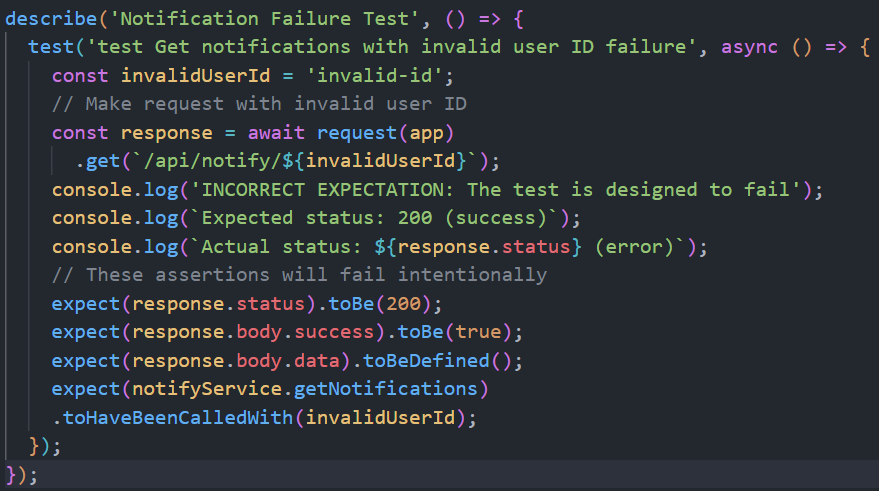
\includegraphics[width=1\textwidth]{figures/consult notifF code.png}
    \caption{Source code of the method consult notifications.}
\end{figure} \
\clearpage
\begin{figure}[h!]
    \centering
    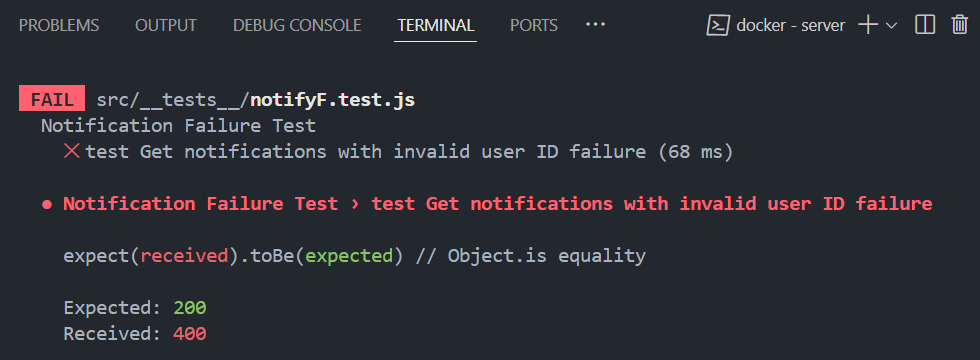
\includegraphics[width=1\textwidth]{figures/result consult notifF.png}  
    \caption{Result of the test consulting notifications}
\end{figure} \


\section{Sprint Review – Burndown Chart Diagram}
The sprint review aims to inspect the results produced during this iteration.
\begin{table}[h!]
\centering
\small
\resizebox{\textwidth}{!}{%
\begin{tabular}{|c|c|c|c|c|c|}
\hline
\textbf{DAY} & \textbf{Hours Planned} & \textbf{Hours Actual} & \textbf{Remaining Planned} & \textbf{Remaining Actual} & \textbf{Done Today} \\
\hline
0  & -  & -  & 160 & 160 & -  \\
1  & 8  & 9  & 152 & 151 & 9  \\
2  & 8  & 10 & 144 & 141 & 10 \\
3  & 8  & 12 & 136 & 129 & 12 \\
4  & 8  & 12 & 128 & 117 & 12 \\
5  & 8  & 8  & 120 & 109 & 8  \\
6  & 8  & 8  & 112 & 101 & 8  \\
7  & 8  & -  & 104 & 101 & -  \\
8  & 8  & 8  & 96  & 93  & 8  \\
9  & 8  & 6  & 88  & 87  & 6  \\
10 & 8  & 5  & 80  & 82  & 5  \\
11 & 8  & 9  & 72  & 73  & 9  \\
12 & 8  & 10 & 64  & 63  & 10 \\
13 & 8  & 10 & 56  & 53  & 10 \\
14 & 8  & 8  & 48  & 45  & 8  \\
15 & 8  & -  & 40  & 40  & -  \\
16 & 8  & 10 & 32  & 35  & 10 \\
17 & 8  & 10 & 24  & 25  & 10 \\
18 & 8  & 7  & 16  & 18  & 7  \\
19 & 8  & 10 & 8   & 10  & 8  \\
20 & 8  & 8  & 0   & 0   & 8  \\
\hline
\end{tabular}%
}
\caption{Tableau de valeurs de Burndown Chart du sprint 2}
\end{table}

\begin{figure}[h!]
    \centering
    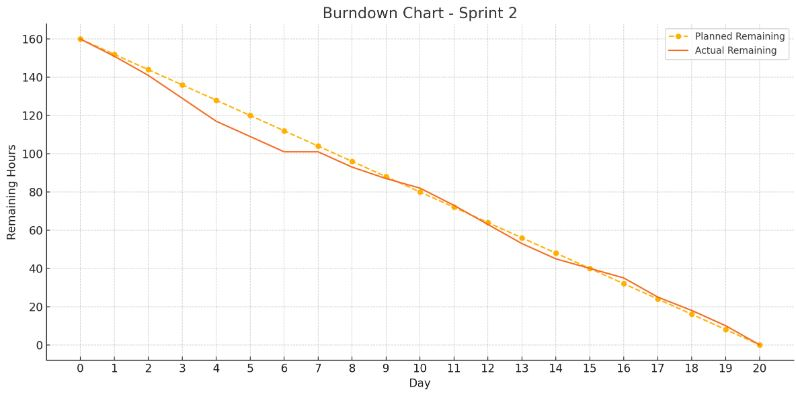
\includegraphics[width=1\textwidth]{figures/burn down chart 2.JPG} 
    \caption{Burn down chart of sprint 2.}
\end{figure} \


\newpage
\begin{center}
    \doublespacing 
    \centering
    \LARGE\textbf{Conclusion} 
    \vspace{1cm} \\
    \raggedright
\end{center}
\addcontentsline{toc}{section}{Conclusion}
In this chapter, we focused on the development of our Second sprint. As a result, we now have a potentially deliverable increment of our platform.
In the next chapter, we will focus on the implementation of our third sprint.



